\documentclass{beamer}
%[aspectratio=169]   \usepackage[czech]{babel}
\usepackage{apo-lecture-en}
\usepackage{pdfpages}
\usepackage{pdfcomment}
\usepackage{listings}
\usepackage{array,multirow}

\subtitle{Lecture 03. Central Processing Unit (CPU)}
\author{Pavel Píša \phantom{xxxxxxx} Petr Štěpán \\ \small\texttt{pisa@fel.cvut.cz} \phantom{xxxx} \small\texttt{stepan@fel.cvut.cz} \\
\phantom{xxxxxxxxx} \\
License: CC-BY-SA}
\begin{document}

\maketitle

\section{Processor}

\begin{frame}
\frametitle{History of QtMips and QtRVSim Simulators}

\begin{itemize}
\item MipsIt used in past for our Computer Architecture course
\item QtMips has been used for APO course from summer term 2019
\begin{itemize}
\item QtMIPS -- master's thesis of Karel Kočí supervised by Pavel Píša: \textit{Graphical CPU Simulator with Cache Visualization}, available at
{\footnotesize \url{https://dspace.cvut.cz/bitstream/handle/10467/76764/F3-DP-2018-Koci-Karel-diploma.pdf}}
\item Fixes, extension and partial internals redesign by Pavel Píša
\end{itemize}
\item Switch to RISC-V architecture in 2022. Main work by Jakub Dupák in 2021, see the master's thesis \textit{Graphical RISC-V Architecture Simulator - Memory Model and Project Management}, available at
{\footnotesize \url{https://dspace.cvut.cz/bitstream/handle/10467/94446/F3-BP-2021-Dupak-Jakub-thesis.pdf}}
\item Alternatives:
\begin{itemize}
 \item RARS: Risc-V Assembler and Runtime Simulator -- IDE with detailed help and hints, evolved from MARS -- \url{https://github.com/TheThirdOne/rars}
 \item EduMIPS64: Java, superscalar pipeline 1x fixed and 3x FP pipelines -- \url{https://www.edumips.org/}
\end{itemize}
\end{itemize}

\end{frame}


\begin{frame}
\frametitle{QtRVSim - Download and Presentations}
\begin{itemize}
\item Windows, Linux, Mac \url{https://github.com/cvut/qtrvsim/releases}
\item  Ubuntu \url{https://launchpad.net/~qtrvsimteam/+archive/ubuntu/ppa}
\item Suse, Fedora and Debian \url{https://software.opensuse.org/download.html?project=home\%3Ajdupak\&package=qtrvsim}
\item Suse Factory TBD
\item Online version \url{https://comparch.edu.cvut.cz/qtrvsim/app/}
\item \textit{QtRvSim - RISC-V Simulator with Cache and Pipeline Visualization}, RISC-V International Academic and Training SIG meeting, 2023, recording \url{https://youtu.be/J6AcPZZ_ISg}
\item \textit{QtRVSim—Education from Assembly to Pipeline, Cache Performance, and C Level Programming}, FOSDEM 2023, Brussels, \url{https://fosdem.org/2023/schedule/event/rv_qtrvsim/}
\end{itemize}
\end{frame}

\begin{frame}[shrink=10]
\frametitle{John von Neumann Computer Block Diagram}
\begin{center}
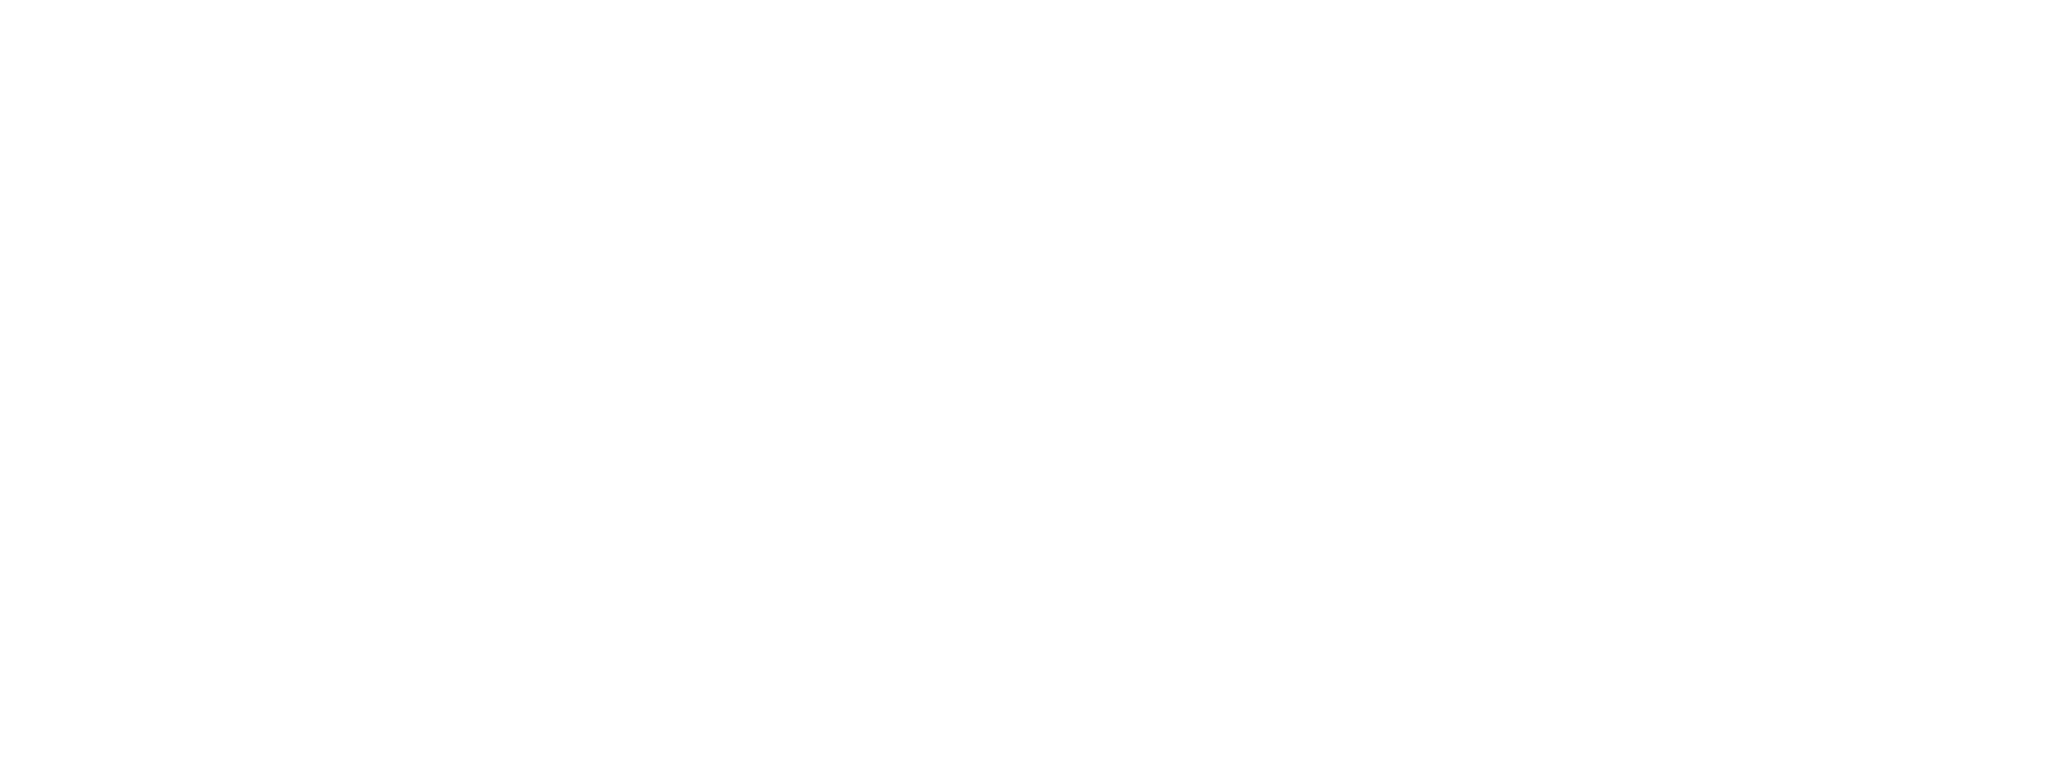
\includegraphics[width=0.5\textwidth]{cpu-vonNeumann.pdf}
%\hfill
%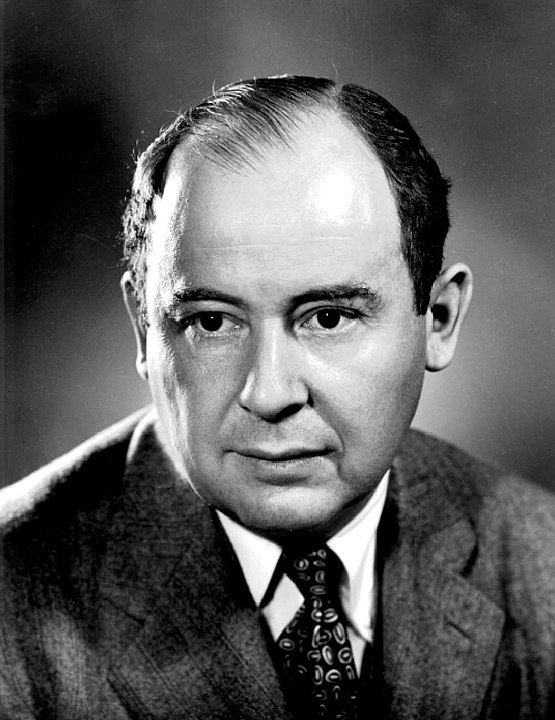
\includegraphics[width=0.15\textwidth]{fig/vonNeumann.png}
\end{center}
\begin{itemize}
\item 5 functional units -- control unit, arithmetic logic unit, memory, input (devices), output (devices)
\item An computer architecture should be independent of solved problems. It has to provide mechanism to load program into memory. The program controls what the computer does with data, which problem it solves.
\item Programs and results/data are stored in the same memory. That memory consists of a cells of same size and these cells are sequentially numbered (address).
\item The instruction which should be executed next, is stored in the cell exactly after the cell where preceding instruction is stored (exceptions branching etc.).
\item The instruction set consists of arithmetics, logic, data movement, jump/branch and special/control instructions.
\end{itemize}
\end{frame}


\begin{frame}
\frametitle{Computer based on von Neumann's concept}

Processor / microprocessor:
\begin{itemize}
\item Control Unit -- CU
\item Arithmetic-Logic Unit -- ALU
\end{itemize}

Memory
\begin{itemize}
\item von Neumann architecture uses common memory, whereas Harvard architecture uses separate program and data memories
\item memory contains cells, i.e., addressable units of same given size (today usually bytes -- 8 bits)
\end{itemize}

Input/output subsystem:
\begin{itemize}
\item Input -- keyboard, mouse
\item Output -- monitors, robotic actuators
\begin{itemize}
\item Today most of peripheral devices functions as both, input, output, network interfaces, disk, SSD, and primarily input or output units has some monitoring and control channels
\end{itemize}
\end{itemize}
\end{frame}


\begin{frame}
\frametitle{Control Unit and Data Path}

The control unit is responsible for control of the operation processing and sequencing. It consists of:
\begin{itemize}
\item control logic circuits which represents core of the control unit (CU)
\item registers -- they hold intermediate and programmer visible state
\end{itemize}

The general purpose registers are used to store actually processed data. For C language programs, they are used to keep some actively processed subset of local variables and temporary values required during expression evaluation.

The flow of instructions and data through processor is usually divided into
\begin{itemize}
\item data path -- the way to load/store data from memory, pass them and retrieve them from registers and to provide them to ALU inputs and then route the results
\item control path -- flow of instruction, their decoding controlling data path according to algorithm
\end{itemize}

\end{frame}


\begin{frame}
\frametitle{The Most Important Registers of Processor}
\begin{itemize}
\item PC (Program Counter) -- holds address of a recent or next instruction to be processed
\item IR (Instruction Register) -- holds the machine instruction read from memory
\item Another usually present registers
\begin{itemize}
\item GPRs (General purpose registers) -- directly under user control, may be divided to address and data or (partially) specialized registers
\item SP (Stack Pointer) -- points to the top of the stack; (The stack is usually used to store local variables and subroutine return addresses)
\item PSW (Program Status Word) -- keeps state as user or system code execution bit etc.
\item IM (Interrupt Mask) -- controls acceptance of asynchronous evens requests
\item FPRs (Floating point registers) -- optional specialized register for hardware floating point real numbers processing
\item more specialize groups possible -- vector registers, multimedia ones, etc.
\end{itemize}
\end{itemize}
\end{frame}

\begin{frame}
\frametitle{The Main Instruction Cycle of the CPU}
\begin{enumerate}
  \item Initial setup/reset -- set initial PC value, PSW, etc.
  \item Read the instruction from the memory
  \begin{itemize}
    \item $PC \to$ to the address bus
    \item Read the memory contents (machine instruction) and transfer it to the IR
    \item $PC+l \to PC$, point $PC$ to next instruction, $l$ is length of actually processed instruction
  \end{itemize}
  \item Decode operation code (opcode)
  \item Execute the operation
  \begin{itemize}
    \item compute effective address, select registers, read operands, pass them through ALU and store result
  \end{itemize}
  \item Check for exceptions/interrupts (and service them) -- more in lecture 9
  \item Repeat from the step 2
\end{enumerate}
\end{frame}


\begin{frame}[fragile,shrink=10]
\frametitle{Compilation: C $\to$ Assembler $\to$ Machine Code}

\begin{columns}
\begin{column}{0.3\textwidth}
\begin{lstlisting}[language={C},columns=flexible]
/* ffs as log2(x)*/
int x = 157;
int y = -1;

while(x != 0) {
  x = x / 2;
  y = y + 1;
}
\end{lstlisting}
\end{column}

\begin{column}{0.35\textwidth}
\begin{lstlisting}[language={C},columns=flexible]
_start:
    // int x = 157;
  addi a0, zero, 157
    // int y = -1;
  addi t1, zero, -1
    // while(x != 0) {
  beq a0, zero, done
loop:
    //   x = x / 2;
  srli a0, a0, 1
    //   y = y + 1;
  addi t1, t1, 1
    // }
  bne a0, zero, loop
done:
\end{lstlisting}
\end{column}

\begin{column}{0.32\textwidth}
\texttt{\phantom{x} \\
\phantom{x} \\
0x00000200:  09d00513\\
\phantom{x} \\
0x00000204:  fff00313\\
\phantom{x} \\
0x00000208:  00050863\\
\phantom{x} \\
\phantom{x} \\
0x0000020c:  00155513\\
\phantom{x} \\
0x00000210:  00130313\\
\phantom{x} \\
0x00000214:  fe051ce3 \\
\phantom{x} }
\end{column}

\end{columns}

\end{frame}

\section{Instruction Encoding}

\begin{frame}
\frametitle{Instruction Encoding Constrains}

Analysis what fits in given instruction length?
\begin{itemize}
\item Idea encode instruction byte, 8 bits, 256 combinations
\begin{itemize}
\item Instruction has to encode operation code (\textbf{opcode}) and operands which should be processed by operation (if not restricted to implicit only)
\item consider 8 registers, 3 bits to encode, two operands instructions only \texttt{$reg_{rsd} = reg_{rsd} + reg_{s1}$} or \texttt{$reg_{rd} = MEM[reg_{s1}]$}
\item 6 bits to select registers $\to$ only 2 bits left $\to$ 4 operations in total
\item that is too small, alternative stack machine with implicit sources on top of stack (usually followed by pop) and implicit destination push to stack top, usually complex
\item extended bytes, immediate operands in byte following opcode and register
\end{itemize}
\item 16-bit instruction encoding, 65536 combinations
\begin{itemize}
\item consider 16 registers, for three operands only 4 bits, 16 two operand instructions left (4 + 3 * 4 bits)
\item usually only two operand (8 + 2 * 4 bits) instructions where 8 bits left for opcode, 256 combinations
\end{itemize}
\end{itemize}
\end{frame}

\begin{frame}
\frametitle{Instruction Encoding Constrains}

\begin{itemize}

\item 32-bit instruction encoding, 4294967296 combinations
\begin{itemize}
\item three operand \texttt{$reg_{rd} = reg_{rs1} + reg_{s2}$} intructions fit
\item common choice 32 registers, and even then 128 thousands three operand instructions (17~+~3~*~5~=~32~bits)
\end{itemize}
\item The immediate values are required as well, add one to register, set register to specific value125
\begin{itemize}
\item but addresses to whole memory are required for global variables for example, if extended instruction words are undesirable, only small offsets (12 or 16 bits) fit
\item the larger ones has to be stored into memory and reverenced by smaller offset which fits into instruction
\item PC relative addressing or addressing against global pointer \textbf{gp}
\item RISC (RISC-V, MIPS, SPARC, POWER, etc.) --  typical fixed length encoding is 32 bits, 12 or 16-bit immediate
\item CISC (x86, m68k) -- instruction variable length encoding, immediate and even registers for extended addressing in followup bytes, words
\end{itemize}
\end{itemize}
\end{frame}


\begin{frame}[shrink=5]
\frametitle{RISC-V -- Instruction Length Encodding}

\begin{tabular}{r l}
  \begin{tabular}{|c|}\hline
  \texttt{xxxxxxxxxxxxxxaa}\\ \hline
  \end{tabular} & 16-bit ($aa \neq 11$)\\
   &  \\
   \begin{tabular}{|c|c|}\hline
  \texttt{xxxxxxxxxxxxxxxx} & \texttt{xxxxxxxxxxxbbb11}\\ \hline
  \end{tabular} & 32-bit ($bbb \neq 111$)\\
 &  \\
   \begin{tabular}{c|c|c|}\hline
  \texttt{...xxxx} &\texttt{xxxxxxxxxxxxxxxx} & \texttt{xxxxxxxxxx011111}\\ \hline
  \end{tabular} & 48-bit\\
 &  \\
   \begin{tabular}{c|c|c|}\hline
  \texttt{...xxxx} &\texttt{xxxxxxxxxxxxxxxx} & \texttt{xxxxxxxxx0111111}\\ \hline
  \end{tabular} & 64-bit\\
 &  \\
   \begin{tabular}{c|c|c|}\hline
  \texttt{...xxxx} &\texttt{xxxxxxxxxxxxxxxx} & \texttt{xnnnxxxxx0111111}\\ \hline
  \end{tabular} & ($80+16\cdot nnn$)-bit\\
  & ($nnn \neq 111$)\\
   \begin{tabular}{c|c|c|}\hline
  \texttt{...xxxx} &\texttt{xxxxxxxxxxxxxxxx} & \texttt{x111xxxxx0111111}\\ \hline
  \end{tabular} & reserved for \\
  & $\ge 192$-bit\\
Address: \phantom{\texttt{yyyyyxxxxxxxxxxxxxxxx    xxxxxxxxx0111111}}&  \\
base+4 \phantom{\texttt{xxxxxxx}} base+2 \phantom{\texttt{xxxxxxxxxxx}} base \phantom{\texttt{xxxxxxx}} &  \\
\end{tabular}

\end{frame}


\begin{frame}[shrink=12]
\frametitle{RISC-V -- Registers}
\begin{tabular}{|l|l|l|l|}\hline
Register & ABI Name & Description & Saver \\ \hline
x0 & zero & Hardwired to zero &  \\\hline
x1 & ra & Return address (from subroutine) & Caller \\\hline
x2 & sp & Stack pointer (for variables and save) &  Callee \\\hline
x3 & gp & Global pointer (base for global data) &  \\\hline
x4 & tp & Thread pointer (thread local store) &  \\\hline
x5-7 & t0--2 & Temporaries (intermediates in computation) &  - \\\hline
x8 & s0/fp & Frame pointer  & Callee \\
   &       & (base for local variable and call frame) &  \\\hline
x9 & s1 & Saved registers (for local variables) &  Callee \\\hline
x10--11 & a0--1 & Function arguments (when function called) &  - \\
 &  & / Return values at end of function  & \\\hline
x12--17 & a2--7 & Function arguments & - \\\hline
x18--27 & s2--11 & Saved registers & Callee \\\hline
x28--31 & t3--6 & Temporaries &  - \\\hline
pc & pc & Program Counter (actual executed instruction) &  \\\hline
f0-31 &  & Floating point registers &  \\\hline
     &  & Machine control and status registers & \\\hline
\end{tabular}
\end{frame}

\begin{frame}
\frametitle{The Goal of This Lecture}

To understand the implementation of a simple computer consisting of CPU and separated instruction and data memory

Our goal is to implement following instructions:

\begin{itemize}
\item Read and write a value from/to the data memory
\begin{itemize}
\item \textbf{\texttt{lw}} -- load word, \textbf{\texttt{sw}} -- store word
\end{itemize}
\item Arithmetic and logic instructions: \textbf{\texttt{add}}, \textbf{\texttt{sub}}, \textbf{\texttt{and}}, \textbf{\texttt{or}}, \textbf{\texttt{slt}}
\begin{itemize}
\item Immediate variants: \textbf{\texttt{addi}}, \textbf{\texttt{ori}}, load of upper bits \textbf{\texttt{lui}},\textbf{\texttt{auipc}}
\end{itemize}
\item Program flow change/jump instruction \textbf{\texttt{beq}}
\item Subroutine call \textbf{\texttt{jal}}, \textbf{\texttt{jalr}} (provides even return from subroutine \textbf{\texttt{jr~ra}})
\item CPU will consist of control unit and ALU (data path).
\item Notes:
\begin{itemize}
\item The implementation will be minimal (single cycle CPU – all operations processed in the single step/clock period)
\item The lecture 5 focuses on more realistic pipelined CPU implementation
\end{itemize}
\end{itemize}

\end{frame}


\begin{frame}
\frametitle{The MIPS Instruction Formats and Instruction Types}

Older but fits into three simple formats:

\begin{tabular}{|c|l|l|l|l|l|l|}\hline
Type & 31 ... 26 & 25 ... 21 & 20 ... 16 & 15 ... 11 & 10 ... 6 & 5 ... 0 \\ \hline
R & opcode(6) & rs(5) & rt(5) & rd(5) & shamt(5) & funct(6) \\ \hline
I & opcode(6) & rs(5) & rt(5) & \multicolumn{3}{c|}{ immediate(16)} \\ \hline
J & opcode(6) & \multicolumn{5}{c|}{ address(26)} \\ \hline
\end{tabular}

\begin{itemize}
\item type (R,I,J) is defined for each 6-bit opcode combination
\item 5 bits allows to encode 32 GPRs (0 / zero is hardwired to 0 / discard)
\item rs -- source register; rd -- destination register; rt -- alternative destination or the second source
\item immediate, address -- encoded direct operand value for ALU or address for branches
\item shamt -- immediate / constant for bit shift operations (\texttt{<<}, \texttt{>>})
\item funct -- for R type specifies ALU operation, addition, subtraction, shift, etc.
\end{itemize}

\end{frame}


\begin{frame}
\frametitle{The RISC-V Instruction Format and Instruction Types}

The six basic formats of the instructions are considered:
\begin{table}
\footnotesize
\begin{tabular}{|m{0.4cm}|m{0.4cm}|m{1.0cm}|m{1.0cm}|m{0.4cm}|m{1.0cm}|m{1.0cm}|m{1.0cm}|m{0.4cm}|m{1.0cm}|}\hline
Type & 31 & 30...25 & 24...21 & 20 & 19...15 & 14...12 & 11...8 & 7 & 6...0 \\ \hline
R & \multicolumn{2}{c|}{ fnct7 } & \multicolumn{2}{c|}{ rs2 } & rs1 & fnct3 &\multicolumn{2}{c|}{ rd } & opcode\\ \hline
I & \multicolumn{4}{c|}{ imm[11:0] } & rs1 & fnct3 &\multicolumn{2}{c|}{ rd } & opcode\\ \hline
S & \multicolumn{2}{c|}{ imm[11:5] } & \multicolumn{2}{c|}{ rs2 } & rs1 & fnct3 &\multicolumn{2}{c|}{ imm[4:0] } & opcode\\ \hline
B & imm [12] & imm [10:5]  & \multicolumn{2}{c|}{ rs2 } & rs1 & fnct3 & imm[4:1]& imm [11] & opcode\\ \hline
U & \multicolumn{6}{c|}{ imm[31:12] }  & \multicolumn{2}{c|}{ rd } & opcode\\ \hline
J & imm [20] & \multicolumn{2}{c|}{ imm[10:1] } & imm [11] & \multicolumn{2}{c|}{ imm[19:12] } & \multicolumn{2}{c|}{ rd } & opcode\\ \hline
\end{tabular}
\end{table}

\begin{itemize}
\item instruction type (R,I,S,B,U,J) and encoding length known from 7-bit \textbf{opcode}
\item rs1, rs2 -- source registers; rd -- destination register
\begin{itemize}
\item the register fields in given role on fixed position for all encodings
\end{itemize}
\item immediate -- directly encoded operands for computation and branches, distributed into unused register fields
\item fnct3, fnct7 -- specifies executed operation (addition, subtraction, shift, etc.) and memory operands width (byte, word, etc.)
\end{itemize}

\end{frame}

\begin{frame}
\frametitle{RISC-V Encoding Codes Overview}

The primary selection of operation is \textbf{opcode}:
\begin{table}
\footnotesize
\begin{tabular}{|c|l|l|}\hline
Opcode & The gorup / operation & Actual operations for our subset \\ \hline
0110011 & R-type (see func7 and func3) & add, sub, slt, or, and \\ \hline
0010011 & ALU-imm. (see func 3) & addi, subi, slti, ori, andi \\ \hline
0000011 & Memory load (func3 with) & lw \\ \hline
0100011 & memory store (func3 width) & sw \\ \hline
1100011 & Branch (func3 condition) & beq \\ \hline
1101111 & Subroutine call & jal \\ \hline
1100111 & Return from subroutine & jalr \\ \hline
0000111 & Load immediate into upper register bits & lui \\ \hline
\end{tabular}
\end{table}

Meaning of \texttt{fnct3} and \texttt{fnct7} for R-type instructions:
\begin{table}
\footnotesize
\begin{tabular}{|l|l|l|}\hline
fnct7 & fnct3 & ALU operation \\ \hline
0000000 & 000  & add \\ \hline
0100000 & 000  & sub \\ \hline
0000000 & 010  & slt \\ \hline
0000000 & 110  & bitwise or \\ \hline
0000000 & 111  & bitwies and \\ \hline
\end{tabular}
\end{table}

\end{frame}

\section{Blocks to Build Processor}

\begin{frame}
\frametitle{Realize Register in Hardware}
Basic realization of register from d-latch circuit
\begin{center}
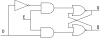
\includegraphics[width=0.5\textwidth]{d_latch.pdf}
\end{center}

This circuit is a big change from the previous approach, because there is a feedback (loop) -- the output of the gate is the input of the same gate, or the input of the other gate whose output is the input of the first gate.

So what does it do?

\end{frame}

\begin{frame}
\frametitle{Realize Register in Hardware}

The circuit actual function is determined by E input (Enable).

Analyze circuit for E=1 the first:
\begin{columns}
\begin{column}{0.5\textwidth}
\begin{center}
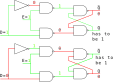
\includegraphics[width=\textwidth]{d_latch_e1-en.pdf}
\end{center}
\end{column}
\begin{column}{0.5\textwidth}
\begin{itemize}
\item The D input propagates Q output after delay
\begin{itemize}
\item when $D=1$ then output has to become $Q=1$, because one of inputs to last gate is 0, and NAND output becomes 1
\item when $D=0$ then output has to become $\overline{Q}=1$, again one input to corresponding NAND gate is 0, when $\overline{Q}=1$, then output $Q=0$, because both inputs of driving gate ate 1, NAND output has to be 0
\end{itemize}
\end{itemize}
\end{column}
\end{columns}

\end{frame}

\begin{frame}
\frametitle{Realize Register in Hardware}

If the enable input is deactivated (E=0):
\begin{columns}
\begin{column}{0.5\textwidth}
\begin{center}
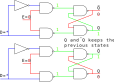
\includegraphics[width=\textwidth]{d_latch_e0-en.pdf}
\end{center}
\end{column}
\begin{column}{0.5\textwidth}
\begin{itemize}
\item The state of $Q,\overline{Q}$ outputs depends only on previous value of $Q,\overline{Q}$
\item The one of states $Q=1,\overline{Q}=0$ or $Q=0,\overline{Q}=1$ is preserved from last situation when $E=1$
\end{itemize}
\end{column}
\end{columns}

\end{frame}

\begin{frame}
\frametitle{Realize Register in Hardware}

Activation by clock signal rising edge:
\begin{columns}
\begin{column}{0.45\textwidth}
\begin{center}
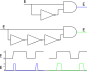
\includegraphics[width=0.9\textwidth]{edge.pdf}
\end{center}
\end{column}
\begin{column}{0.55\textwidth}
\begin{itemize}
\item Is it possible that output of such circuit reaches active (1) state?
\item for ideal/matthematic case no $(C$~and~$\overline{C})=0$
\item in reality, however, the gate output is delayed compared to the direct bypass signal and for this delay time the output is \texttt{E'} v 1
\end{itemize}
\end{column}
\end{columns}
\bigskip
\begin{itemize}
\item if this value is too short compared to the d-latch circuit settle time, then it is possible to add more consecutive negations (green curve)
\item the variant of sequential circuit which state is recorded at clock signal edge is called d flip-flop
\end{itemize}

\end{frame}


\begin{frame}
\frametitle{Hardware Realization of CPU Instruction Cycle}

\begin{center}
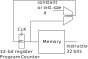
\includegraphics[width=0.55\textwidth]{cpu_step-en.pdf}
\end{center}

The PC register is updated to PC+4 (advanced by instruction length) at clock (CLK) signal rising edge which causes start of the fetch of following instruction from memory.
\end{frame}

\begin{frame}
\frametitle{Processor Basic Building Blocks}

\begin{table}
\footnotesize
\begin{tabular}{m{1.6cm} m{9.5cm}}
\hfill 
\includegraphics[width=0.6cm]{registr.pdf} & single 32-bit wide register, the input store at CLK rising edge \\
\phantom{X} & \phantom{X} \\
\hfill 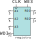
\includegraphics[width=1.6cm]{registry.pdf} & 32 registers in register file, A1, A2 inputs select which register values are connected to RD1 and RD2 outputs; if WE3 (write enable) insputs is active then WD3 input state is written to register designated by A3 at CLK signal rising edge \\
\phantom{X} & \phantom{X} \\
\hfill 
\includegraphics[width=0.8cm]{multiplexor.pdf} & multiplexer copies one of its input signals to the output according to Select input value \\
\phantom{X} & \phantom{X} \\
\hfill 
\includegraphics[width=1.2cm]{alu.pdf} & the operation chosen by ALUControl signal is applied to inputs SrcA and SrcB. Result is available on ALUout signal and flags reflects result conditions, i.e., sign or indicate zero value\\
\phantom{X} & \phantom{X} \\
\hfill 
\includegraphics[width=1.6cm]{imm_decode.pdf} & chooses bits used for immediate encoding and applies sign extension to 32 bits signed value \\
\end{tabular}
\end{table}

\end{frame}


\begin{frame}
\frametitle{Processor Basic Building Blocks -- Memory}

\begin{table}
\footnotesize
\begin{tabular}{m{2.2cm} m{9.0cm}}
\hfill 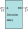
\includegraphics[width=2cm]{inst_mem-en.pdf} & Instruction memory provides data stored in the memory cell/word indexed by address input A on its output RD. Data are available after interval "long enough" to stabilize address decoder and propagate value to the output RD (the read access time).\\
\phantom{X} & \phantom{X} \\
\hfill 
\includegraphics[width=2.4cm]{memory-en.pdf} & Data memory. In read mode, it delivers memory cell/word content indexed bay address A onto RD output (again read access time has to be respected). If the input WE (write enable) is active then data stable for long enough setup time are stored into selected word at rising edge of the clock (CLK). The time from data and address ready to stable data writes into cell is called write access time.\\
\end{tabular}
\end{table}

\end{frame}


\section{Simple Single Cycle CPU Incremental Design}

\begin{frame}
\frametitle{The Load Word Instruction - LW}

\textbf{\texttt{lw} -- \texttt{load word}} -- load word from data memory into a register

\begin{tabular}{|l|l|}\hline
Description & A word is loaded into a register from the specified address \\ \hline
Operation & \texttt{[rd]} $\leftarrow$ \texttt{Mem[[rs1]+imm12]} \\ \hline
Syntax & lw rd, imm12(rs1) \\ \hline
Encoding & \texttt{iiii iiii iiii ssss s010 dddd d000 0011} \\ \hline
 & s -- rs1; d -- rd; i -- immediate \\ \hline
\end{tabular}

\bigskip

Example: Reads 32-bit word stored at address 0x400 in memory into register 2:\\
\textbf{\texttt{lw x2, 0x400(x0)}}

\textbf{\texttt{\color{red}iiii iiii iiii}}\phantom{xx}\textbf{\texttt{\color{blue}ssss s}}\hspace{0.1cm}\textbf{\texttt{010\hspace{0.25cm}{\color{green}dddd d}\hspace{0.05cm}000 0011}}\\
$\underbrace{\textbf{\texttt{\color{red}0100 0000 0000}}}_{0x400}\texttt{ }\underbrace{\textbf{\texttt{\color{blue}0000 0}}}_{0}\underbrace{\textbf{\texttt{010}}}_{func3}\phantom{i}\underbrace{\textbf{\texttt{\color{green}0001 0}}}_{2}\underbrace{\textbf{\texttt{000 0011}}}_{opcode}$\\

\textbf{\texttt{0x 40 00 21 03}} -- machine code \textbf{\texttt{lw x2, 0x400(x0)}}

Remark: x0 register provides fixed zero value which is not changed even by write

\end{frame}

\begin{frame}[shrink=15]
\frametitle{The Load Word Instruction -- Implementation}

\textbf{\texttt{lw}}: \texttt{rs1} -- base address, \texttt{imm12} -- address offset, \texttt{rd} -- register where to store fetched data

\bigskip

\begin{table}
\footnotesize
\begin{tabular}{|m{0.4cm}|m{0.4cm}|m{1.0cm}|m{1.0cm}|m{0.4cm}|m{1.0cm}|m{1.0cm}|m{1.0cm}|m{0.4cm}|m{1.0cm}|}\hline
Typ & 31 & 30...25 & 24...21 & 20 & 19...15 & 14...12 & 11...8 & 7 & 6...0 \\ \hline
I & \multicolumn{4}{c|}{ imm[11:0] } & rs1 & fnct3 &\multicolumn{2}{c|}{ rd } & opcode\\ \hline
\end{tabular}
\end{table}

\bigskip

\begin{center}
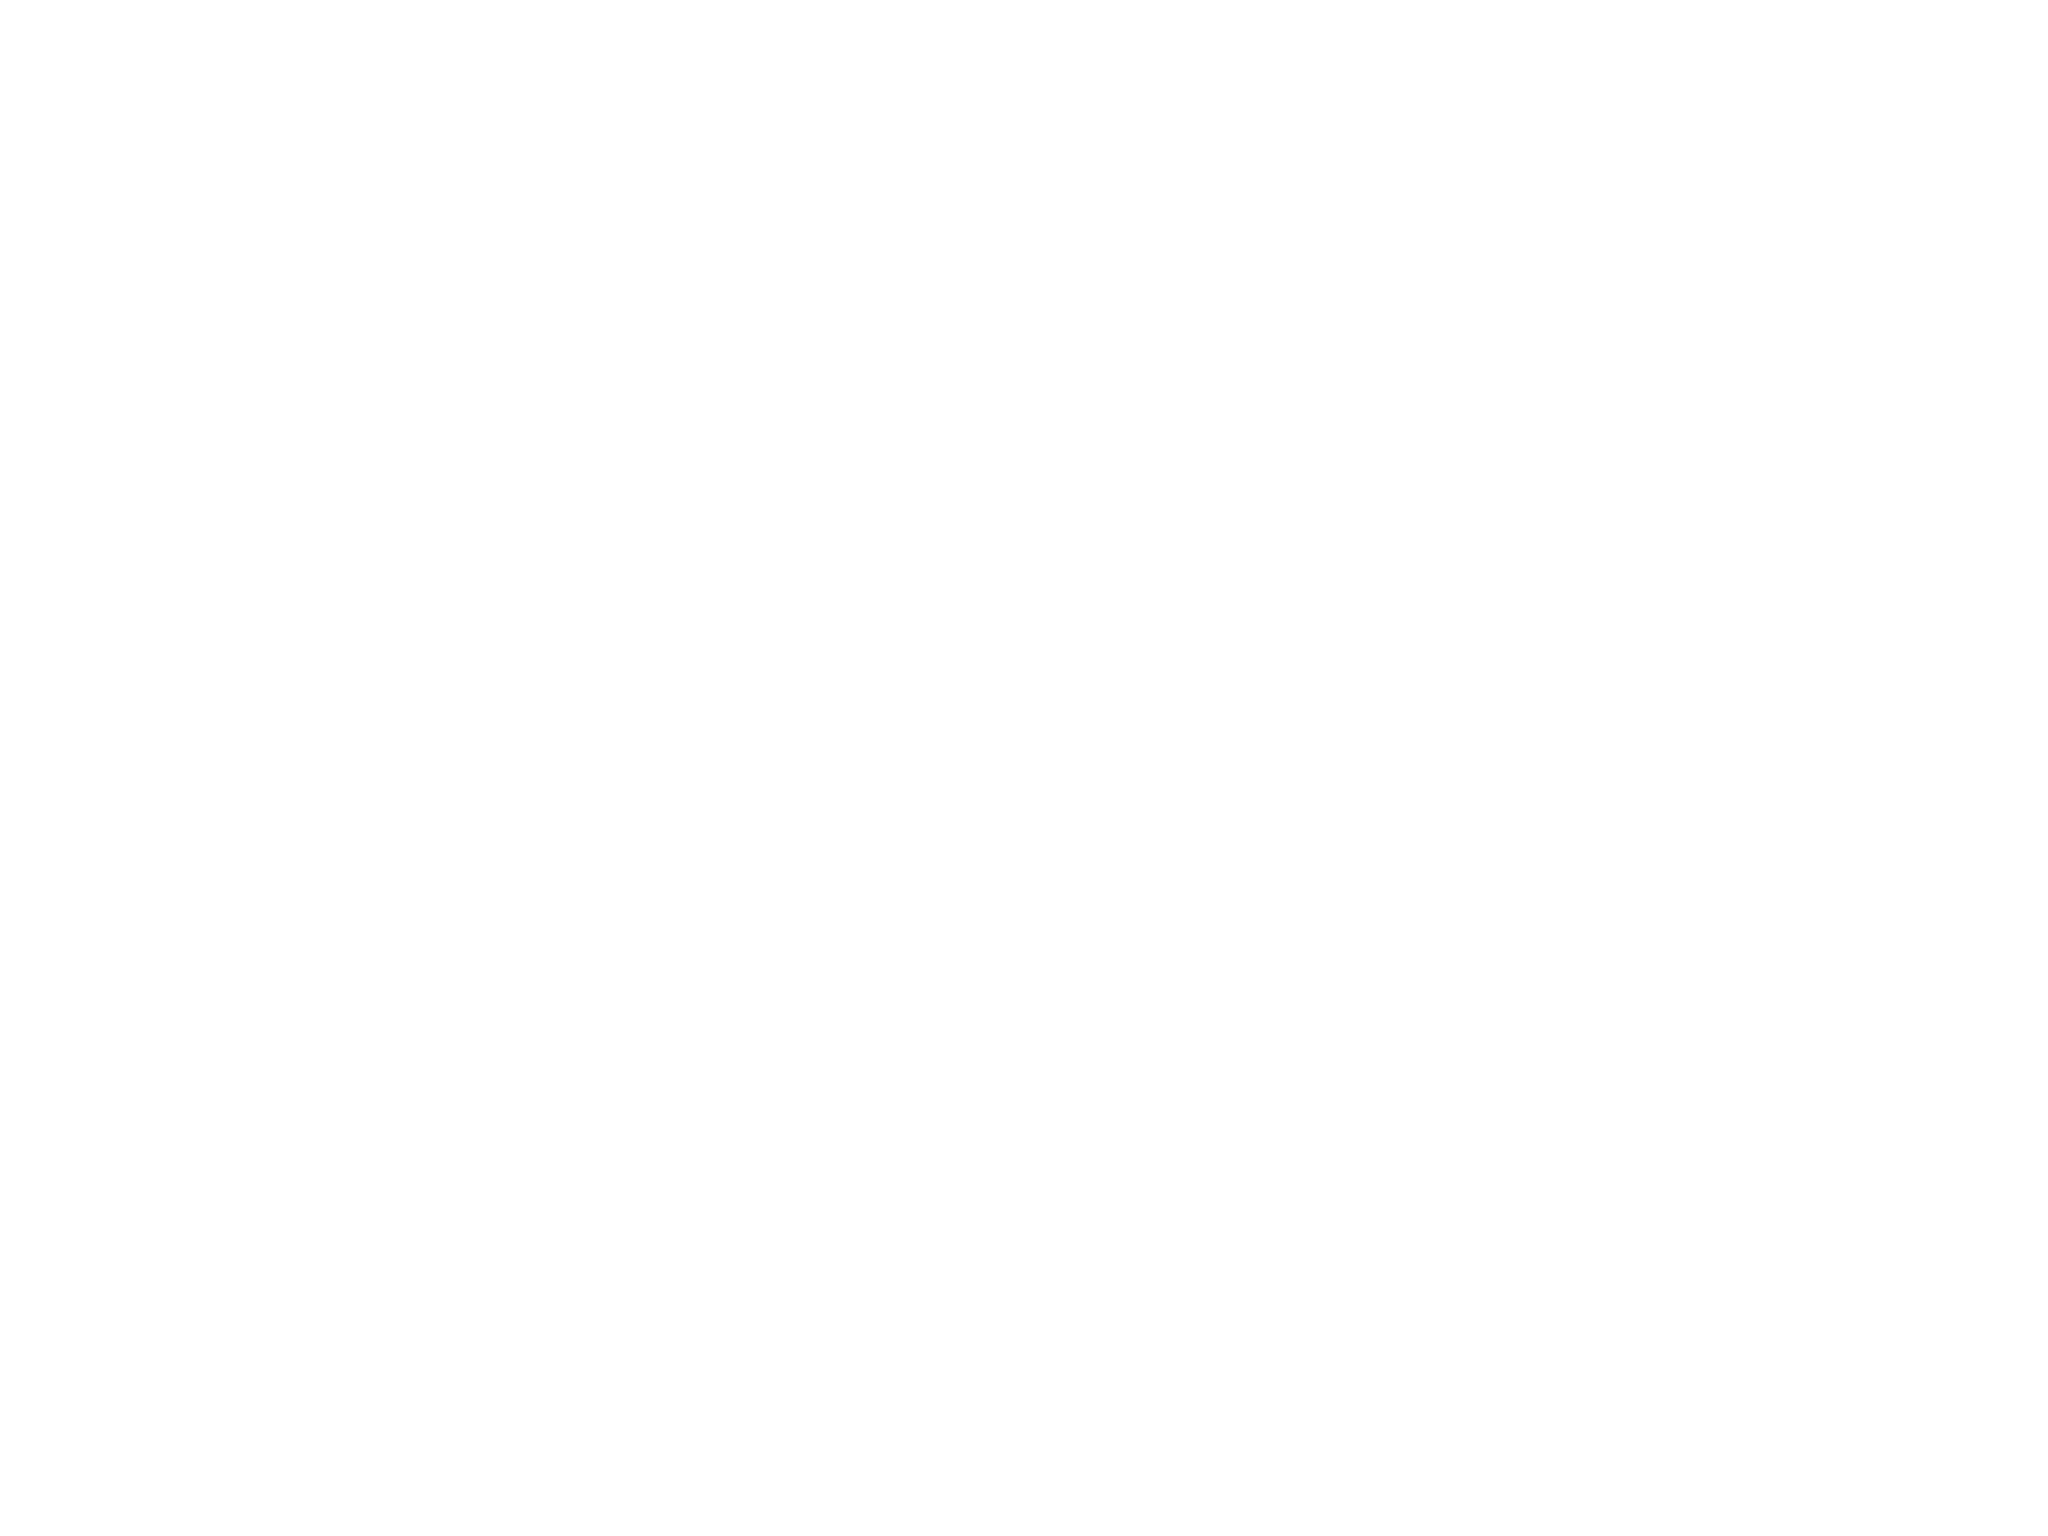
\includegraphics[width=0.85\textwidth]{cpu-load.pdf}
\end{center}

\end{frame}

\begin{frame}[shrink=15]
\frametitle{The Load Word Instruction -- Implementation}

\textbf{\texttt{lw}}: \texttt{rs1} -- base address, \texttt{imm12} -- address offset, \texttt{rd} -- register where to store fetched data

\bigskip

\begin{table}
\footnotesize
\begin{tabular}{|m{0.4cm}|m{0.4cm}|m{1.0cm}|m{1.0cm}|m{0.4cm}|m{1.0cm}|m{1.0cm}|m{1.0cm}|m{0.4cm}|m{1.0cm}|}\hline
Typ & 31 & 30...25 & 24...21 & 20 & 19...15 & 14...12 & 11...8 & 7 & 6...0 \\ \hline
I & \multicolumn{4}{c|}{ imm[11:0] } & rs1 & fnct3 &\multicolumn{2}{c|}{ rd } & opcode\\ \hline
\end{tabular}
\end{table}

Write to register at the rising edge of the clock

\begin{center}
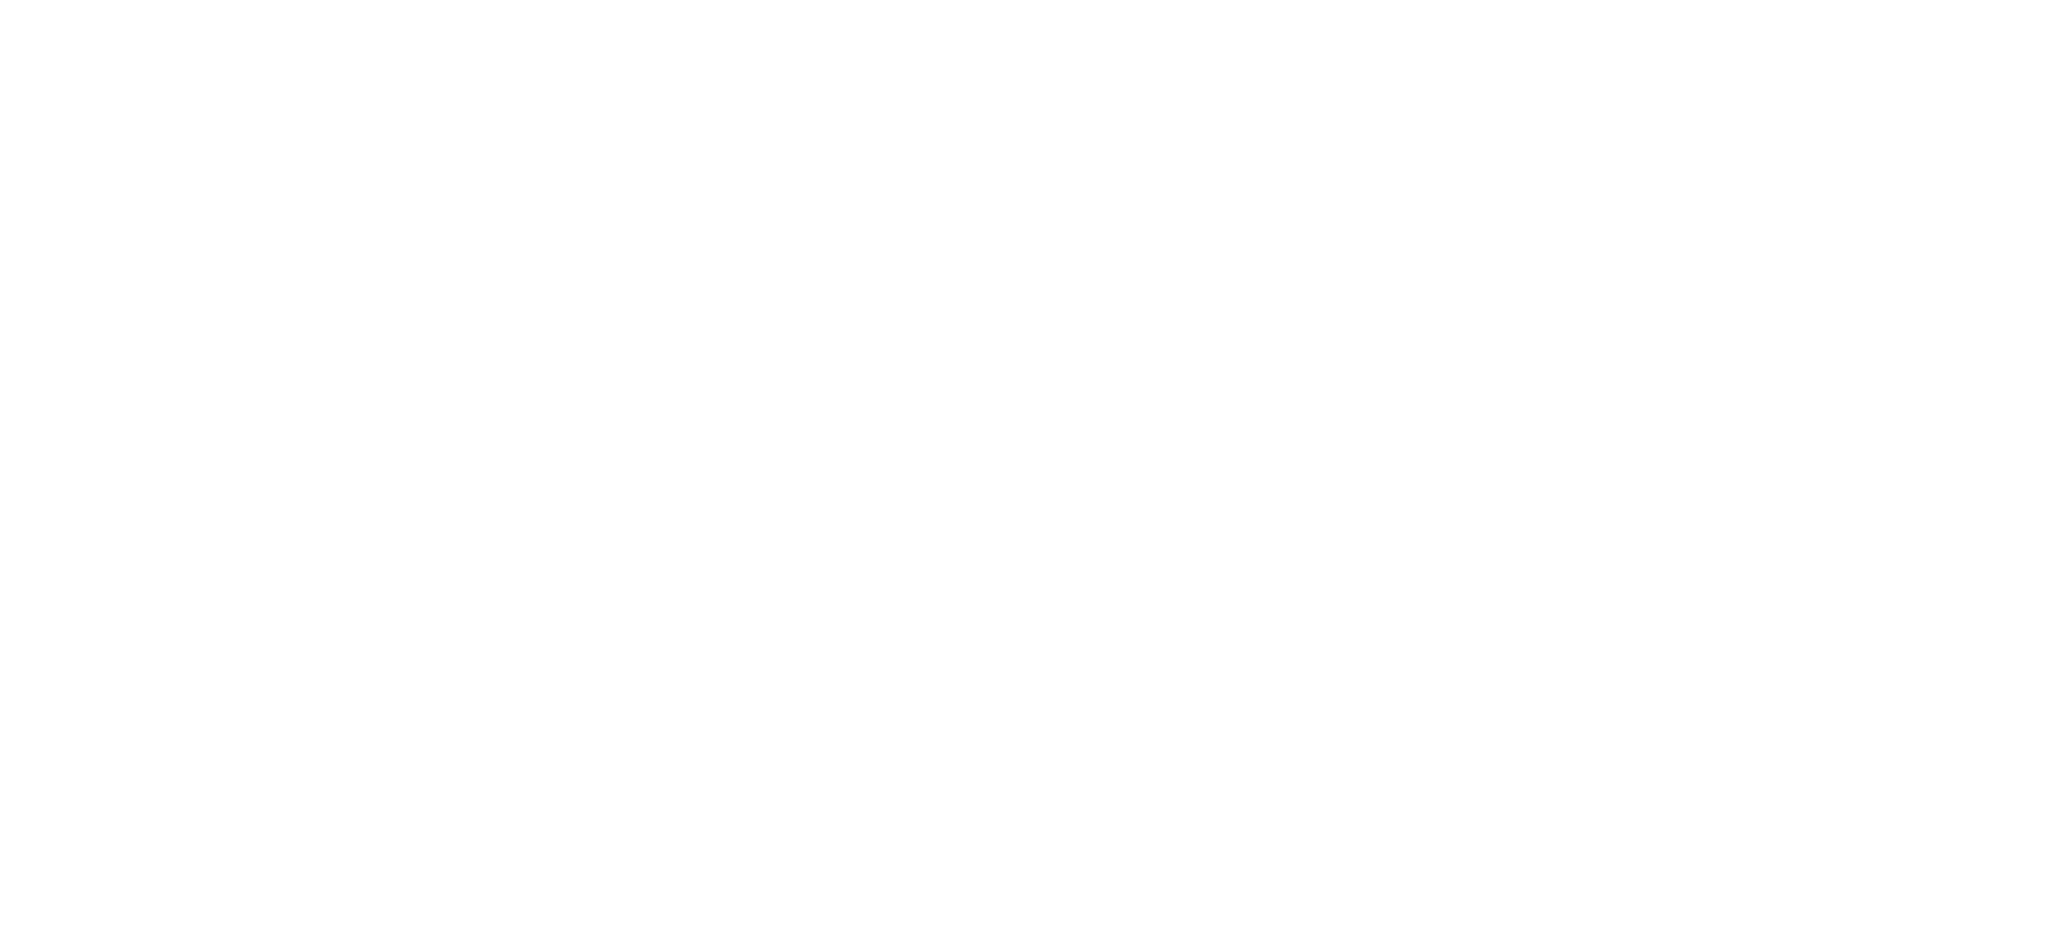
\includegraphics[width=0.90\textwidth]{cpu-load-red.pdf}
\end{center}

\end{frame}


\begin{frame}[shrink=15]
\frametitle{The Load Word Instruction -- Implementation}

\textbf{\texttt{lw}}: \texttt{rs1} -- base address, \texttt{imm12} -- address offset, \texttt{rd} -- register where to store fetched data

\bigskip

\begin{table}
\footnotesize
\begin{tabular}{|m{0.4cm}|m{0.4cm}|m{1.0cm}|m{1.0cm}|m{0.4cm}|m{1.0cm}|m{1.0cm}|m{1.0cm}|m{0.4cm}|m{1.0cm}|}\hline
Typ & 31 & 30...25 & 24...21 & 20 & 19...15 & 14...12 & 11...8 & 7 & 6...0 \\ \hline
I & \multicolumn{4}{c|}{ imm[11:0] } & rs1 & fnct3 &\multicolumn{2}{c|}{ rd } & opcode\\ \hline
\end{tabular}
\end{table}

\bigskip

\begin{center}
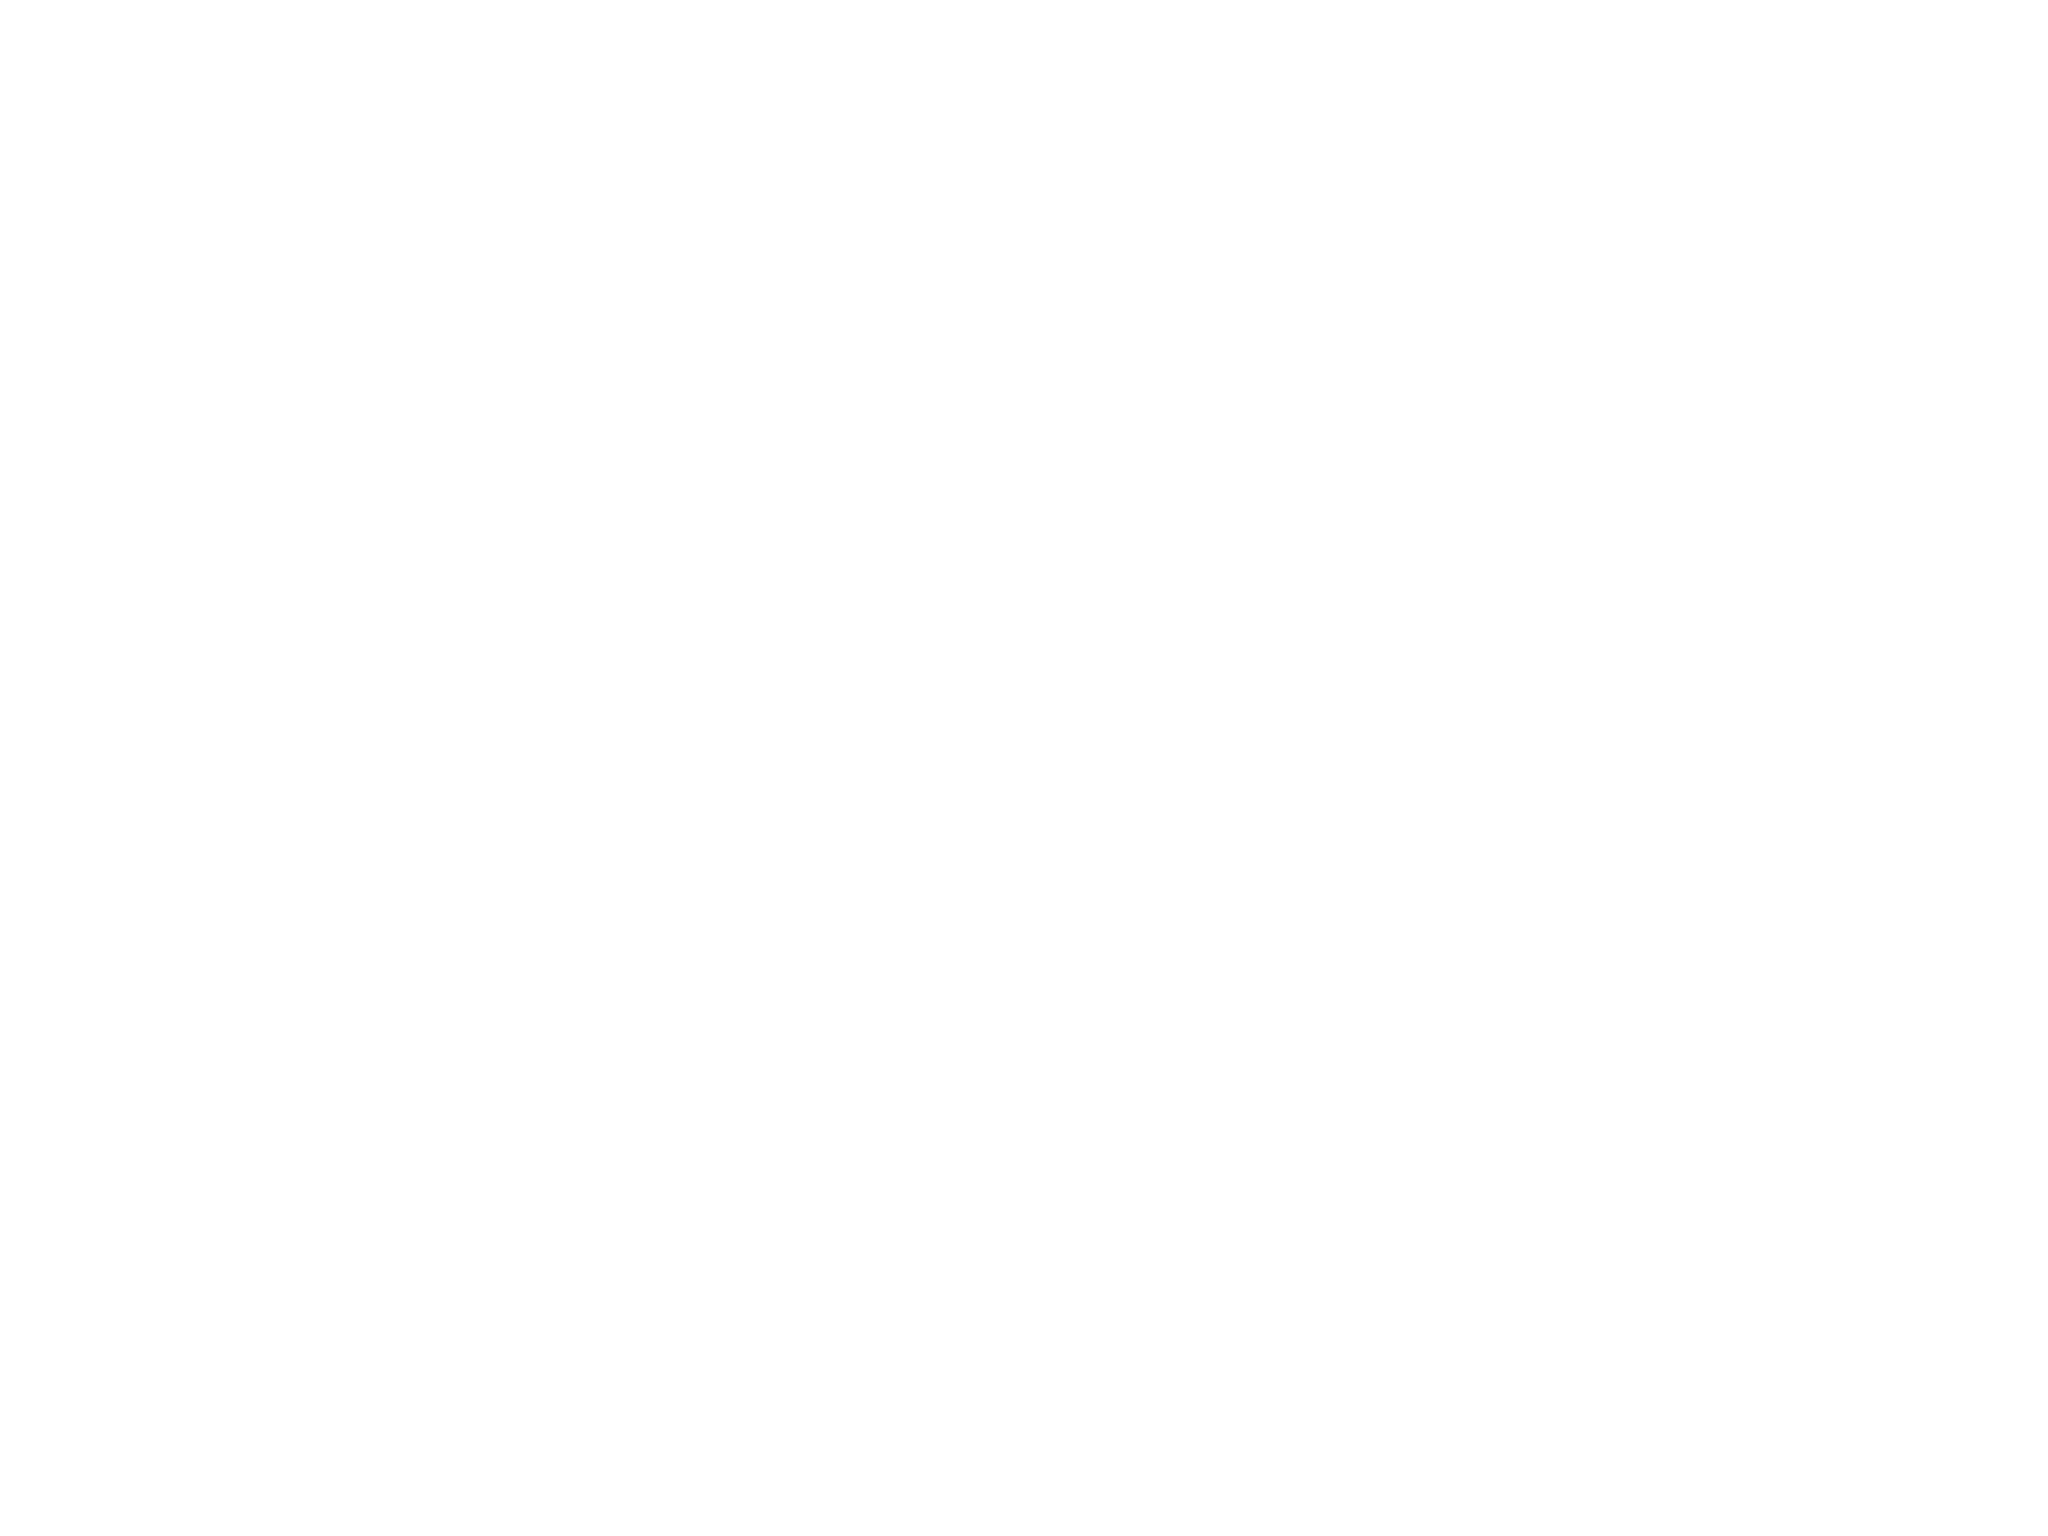
\includegraphics[width=0.88\textwidth]{cpu-load2.pdf}
\end{center}
\end{frame}


\begin{frame}
\frametitle{QtRvSim - RISC-V Simultaor}

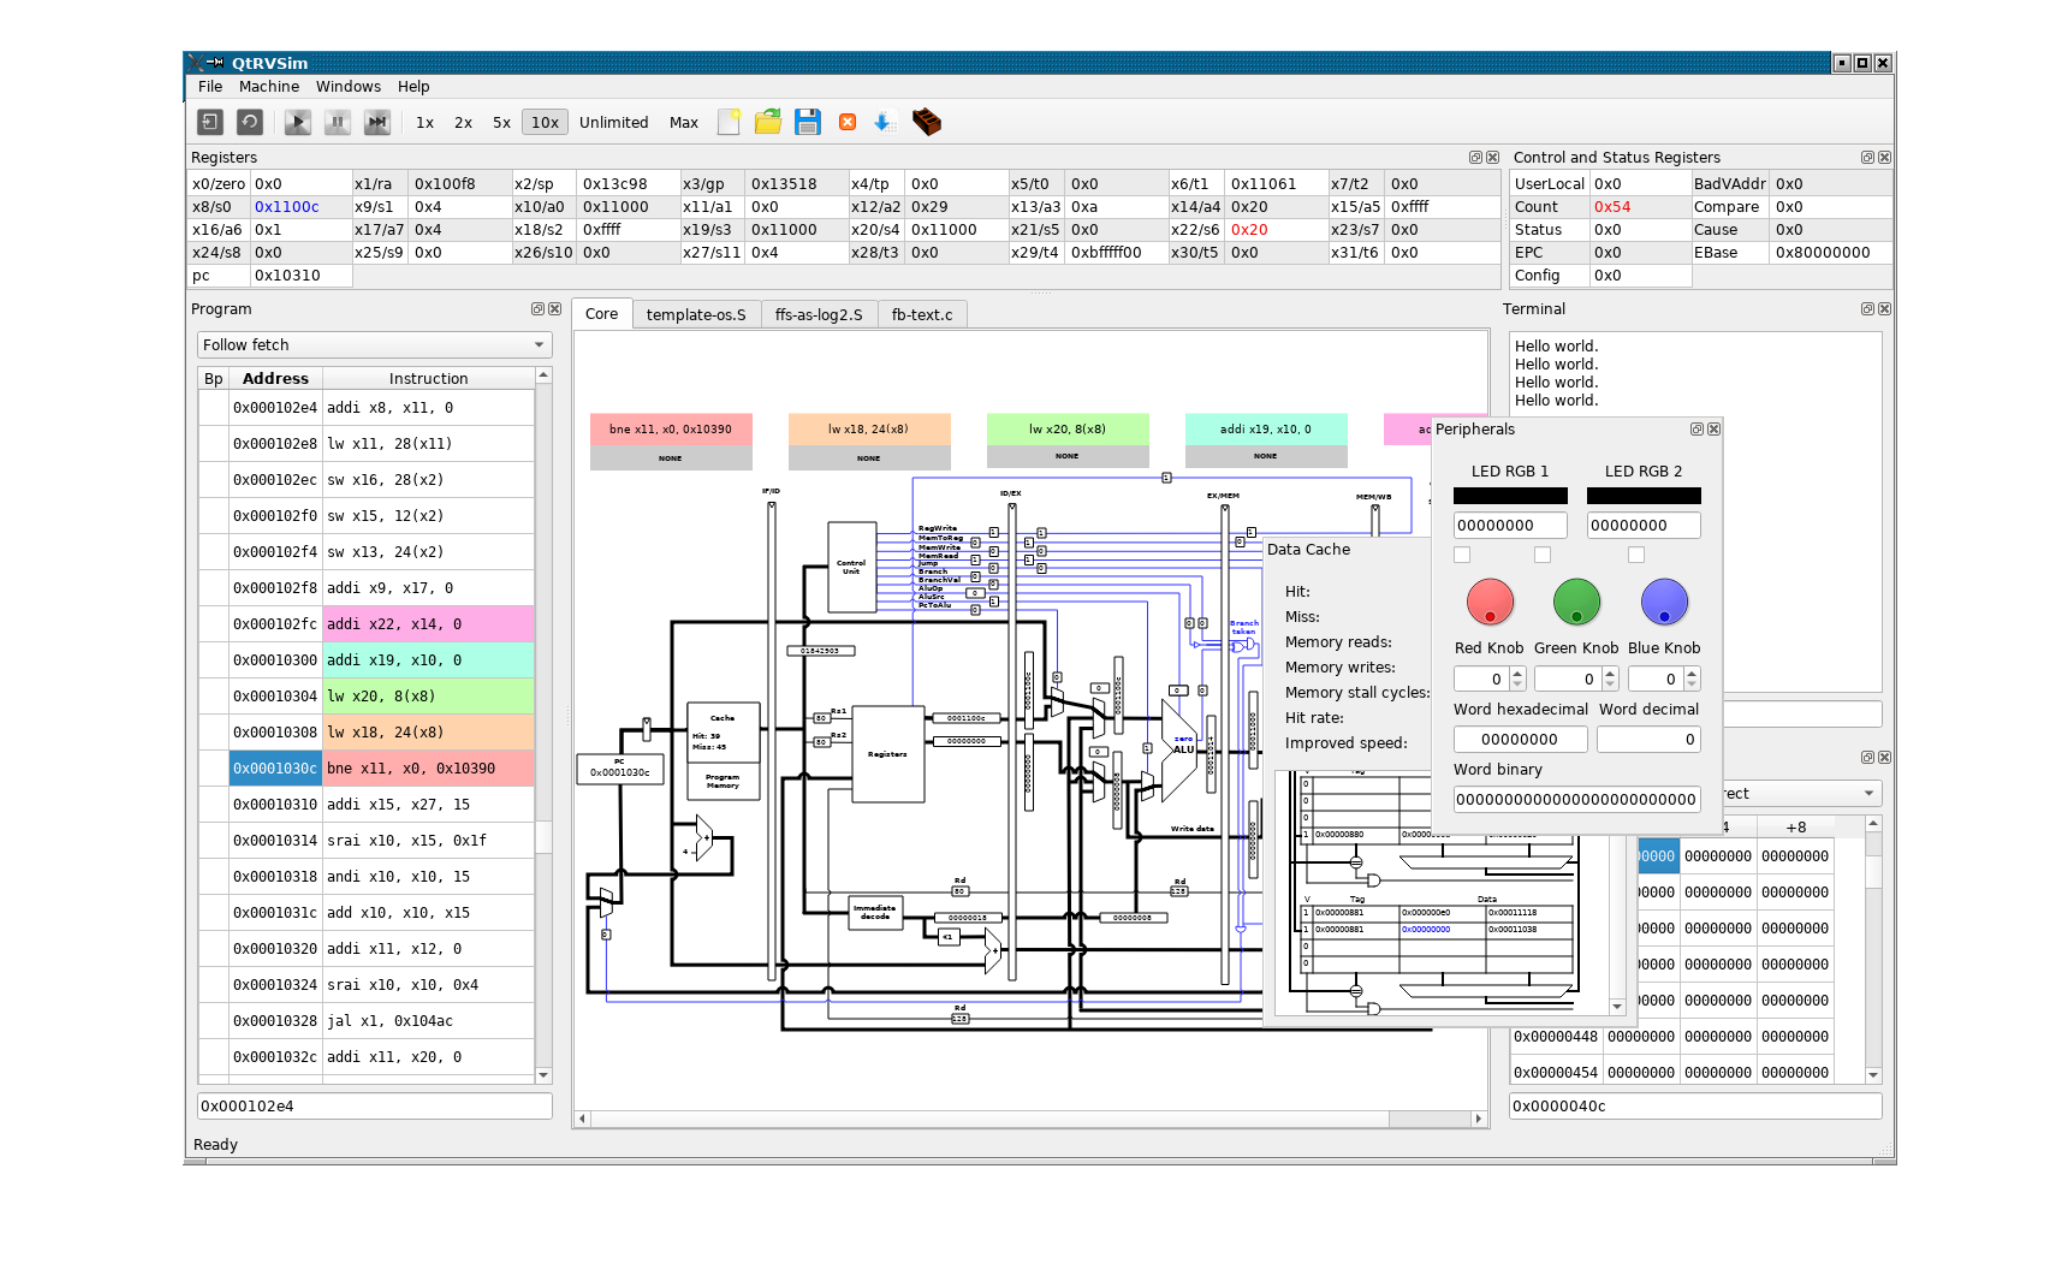
\includegraphics[width=0.9\textwidth]{simulator.pdf}

\end{frame}



\begin{frame}
\frametitle{The Store Word Instruction - SW}

\textbf{\texttt{sw} -- \texttt{store word}} --  store word in a register to data memory

\bigskip

\begin{tabular}{|l|l|}\hline
Description & Stores a value in register rs2 to given address in memory \\ \hline
Operation& \texttt{Mem[[rs1]+imm12]} $\leftarrow$ \texttt{[rs2]} \\ \hline
Syntax & sw rs2, imm12(rs1) \\ \hline
Encoding & \texttt{iiii iiit tttt ssss s010 iiii i010 0011} \\
 & t -- rs2; s -- rs1; i -- immediate \\ \hline
\end{tabular}

\bigskip

Example: Store word in register 2 to memory address computed as addition of value in register 5 and constant 0x404, bit symbol \texttt{t} used for rs2:\\
\textbf{\texttt{sw x2, 0x404(x5)}}

\textbf{\texttt{{\color{green}iiii iii}\hspace{0.08cm}\color{red}t tttt}}\phantom{x}\hspace{0.13cm}\textbf{\texttt{\color{blue}ssss s}}\hspace{0.1cm}\textbf{\texttt{010\hspace{0.25cm}{\color{green}iiii i}\hspace{0.05cm}010 0011}}\\
$\underbrace{\textbf{\texttt{\color{green}0100 000}}}_{0x40\_}
\underbrace{\textbf{\texttt{\color{red}0 0010}}}_{2}
\texttt{ }\underbrace{\textbf{\texttt{\color{blue}0010 1}}}_{5}
\underbrace{\textbf{\texttt{010}}}_{func3}\phantom{i}\underbrace{\textbf{\texttt{\color{green}0010 0}}}_{0x \_04}
\underbrace{\textbf{\texttt{010 0011}}}_{opcode}$\\

\textbf{\texttt{0x 40 22 a2 23}} -- machine code \textbf{\texttt{sw x2, 0x404(x5)}}

\end{frame}

\begin{frame}[shrink=18]
\frametitle{The Store Word Instruction -- Implementation}

\textbf{\texttt{sw}}: \texttt{rs1} -- base address, \texttt{imm12} -- address offset, \texttt{rs2} -- selects register to store into memory

\bigskip

\begin{table}
\footnotesize
\begin{tabular}{|m{0.4cm}|m{0.4cm}|m{1.0cm}|m{1.0cm}|m{0.4cm}|m{1.0cm}|m{1.0cm}|m{1.0cm}|m{0.4cm}|m{1.0cm}|}\hline
Typ & 31 & 30...25 & 24...21 & 20 & 19...15 & 14...12 & 11...8 & 7 & 6...0 \\ \hline
S & \multicolumn{2}{c|}{ imm[11:5] } & \multicolumn{2}{c|}{ rs2 } & rs1 & fnct3 &\multicolumn{2}{c|}{ imm[4:0] } & opcode\\ \hline
\end{tabular}
\end{table}

\bigskip

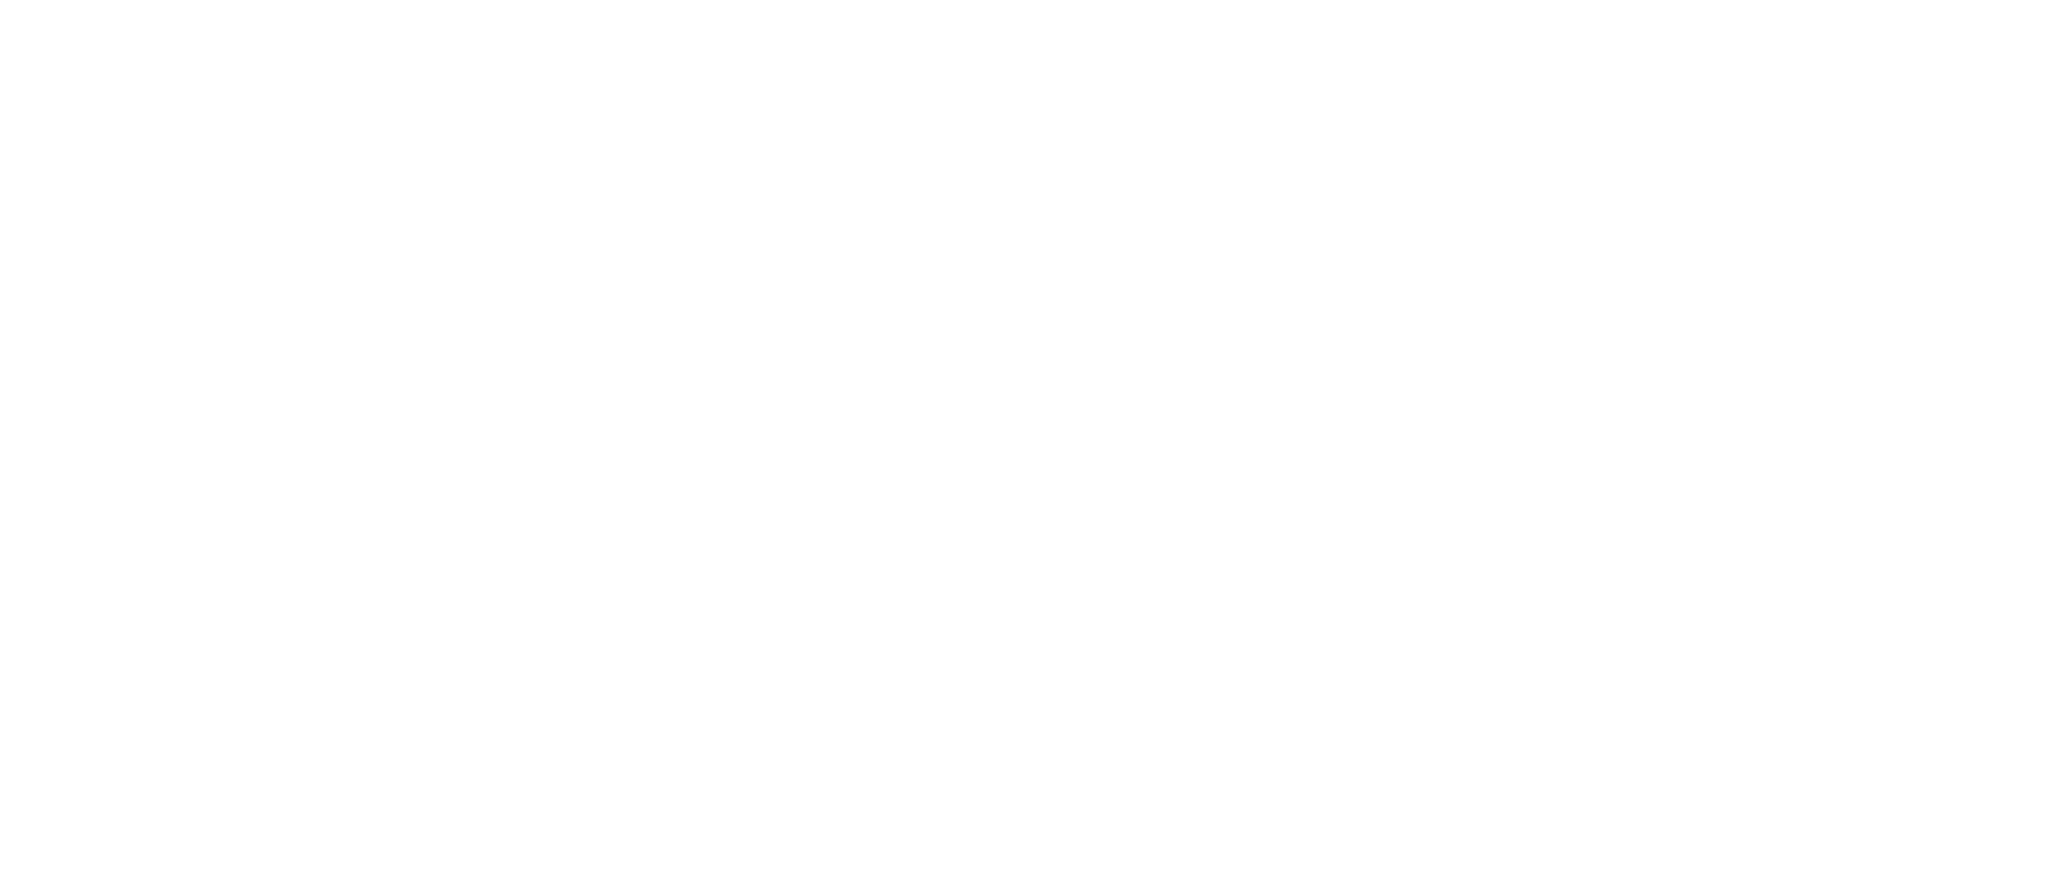
\includegraphics[width=0.90\textwidth]{cpu-store2.pdf}

\end{frame}




\begin{frame}
\frametitle{Instruction for Two Registers Addition -- ADD}

\textbf{\texttt{add} -- \texttt{addition}} -- add content of two registers and store it to destination one

\bigskip

\begin{tabular}{|l|l|}\hline
Description & Add together values in two registers (rs1 + rs2) \\
            & and stores the result in register rd \\ \hline
Operation& \texttt{[rd]} $\leftarrow$ \texttt{[rs1] + [rs2]} \\ \hline
Syntax & add rd, rs1, rs2 \\ \hline
Encoding & \texttt{0000 000t tttt ssss s010 dddd d011 0011} \\
 & t -- rs2; s -- rs1; d -- rd \\ \hline
\end{tabular}

\bigskip

Example: Add values in registers 2 and 3 and store result into register 4:\\
\textbf{\texttt{add x4, x2, x3}}

\textbf{\texttt{0000 000\hspace{0.08cm}\color{red}t tttt}}\phantom{x}\hspace{0.13cm}\textbf{\texttt{\color{blue}ssss s}}\hspace{0.1cm}\textbf{\texttt{000\hspace{0.25cm}{\color{green}dddd d}\hspace{0.05cm}011 0011}}\\
$\underbrace{\textbf{\texttt{0000 000}}}_{funct7}
\underbrace{\textbf{\texttt{\color{red}0 0011}}}_{3}
\texttt{ }\underbrace{\textbf{\texttt{\color{blue}0001 0}}}_{2}
\underbrace{\textbf{\texttt{000}}}_{func3}\phantom{i}
\underbrace{\textbf{\texttt{\color{green}0010 0}}}_{4}
\underbrace{\textbf{\texttt{011 0011}}}_{opcode}$\\

\textbf{\texttt{0x 00 31 02 33}} -- machine code \textbf{\texttt{add x4, x2, x3}}


\end{frame}

\begin{frame}[shrink=25]
\frametitle{Two Registers Addition -- Implementation}

\textbf{\texttt{add}}: \texttt{rs1}, \texttt{rs2} -- sources, \texttt{rd} -- destination register to store result

\bigskip

\begin{table}
\footnotesize
\begin{tabular}{|m{0.4cm}|m{0.4cm}|m{1.0cm}|m{1.0cm}|m{0.4cm}|m{1.0cm}|m{1.0cm}|m{1.0cm}|m{0.4cm}|m{1.0cm}|}\hline
Typ & 31 & 30...25 & 24...21 & 20 & 19...15 & 14...12 & 11...8 & 7 & 6...0 \\ \hline
R & \multicolumn{2}{c|}{ fnct7 } & \multicolumn{2}{c|}{ rs2 } & rs1 & fnct3 &\multicolumn{2}{c|}{ rd } & opcode\\ \hline
\end{tabular}
\end{table}

\bigskip

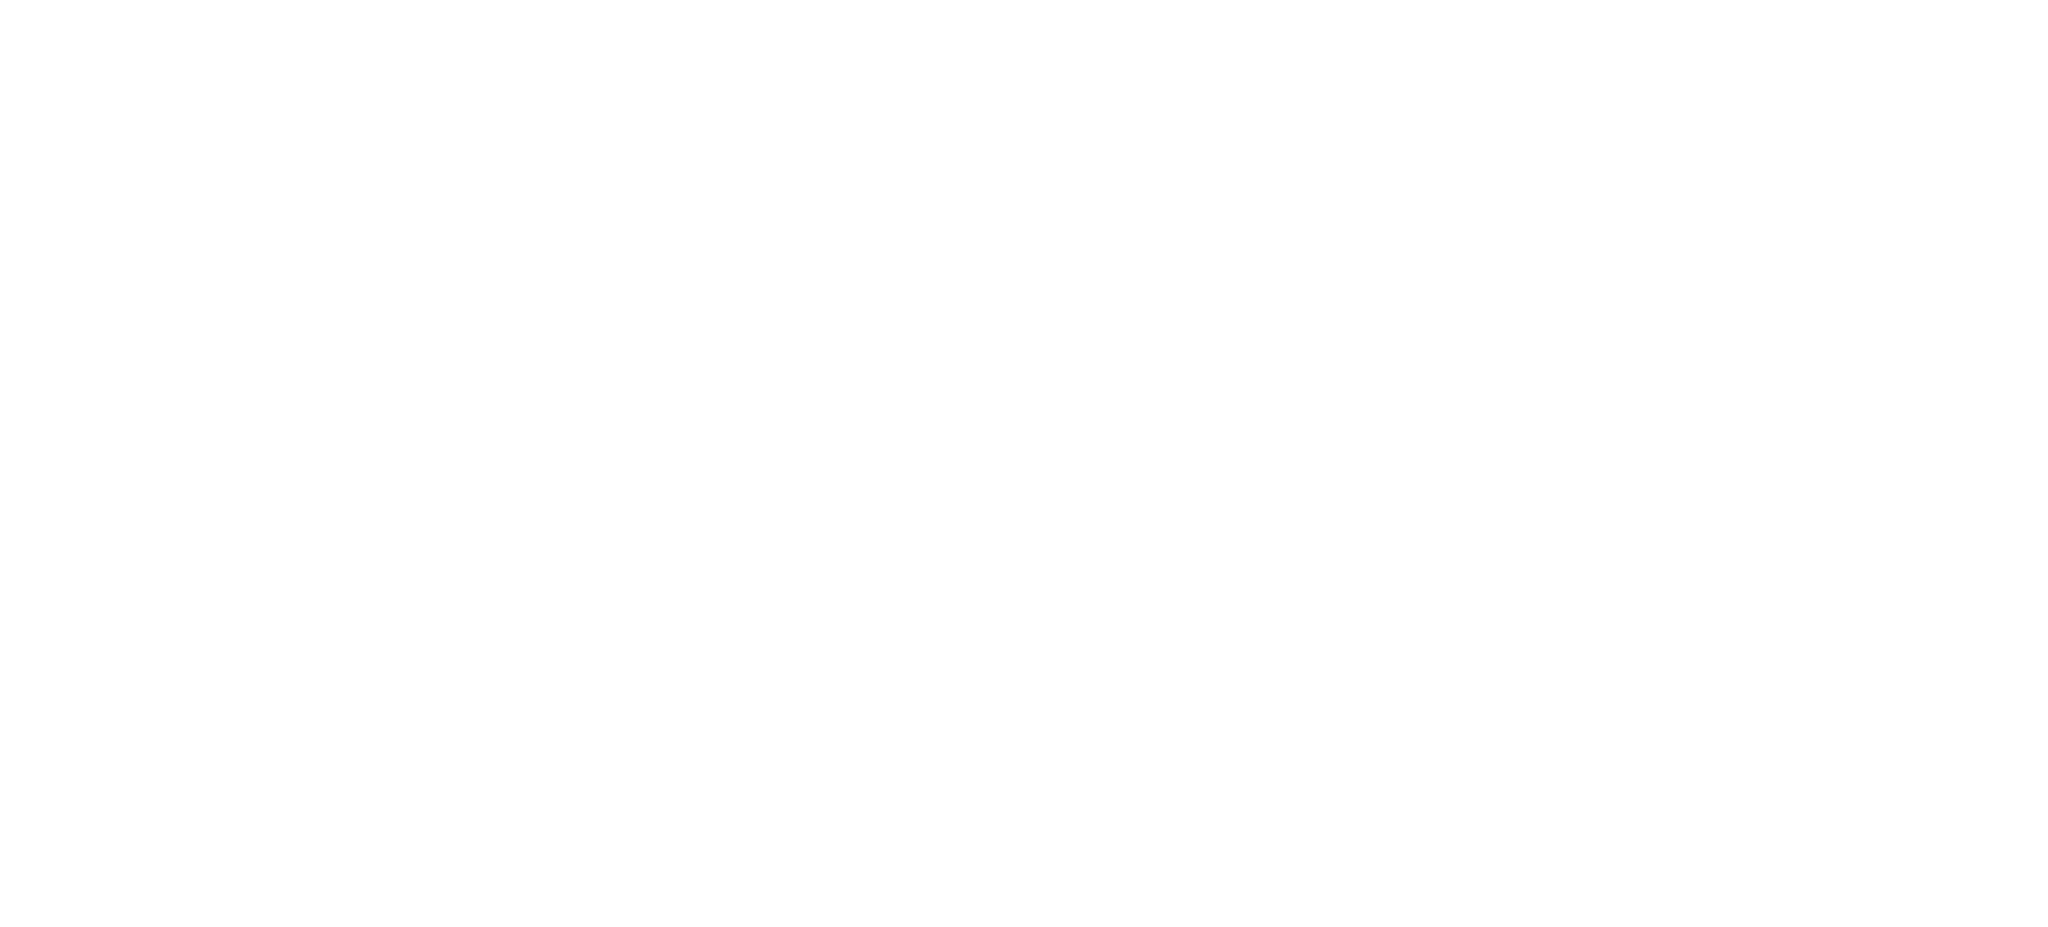
\includegraphics[width=0.85\textwidth]{cpu-add.pdf}

\end{frame}


\begin{frame}
\frametitle{More Arithmetic Instructions -- SUB, AND, OR, SLT}

Another ALU operation selection (ALUcontrol) is only difference to addition. The data path is the same as for add instruction.
\bigskip

\bigskip

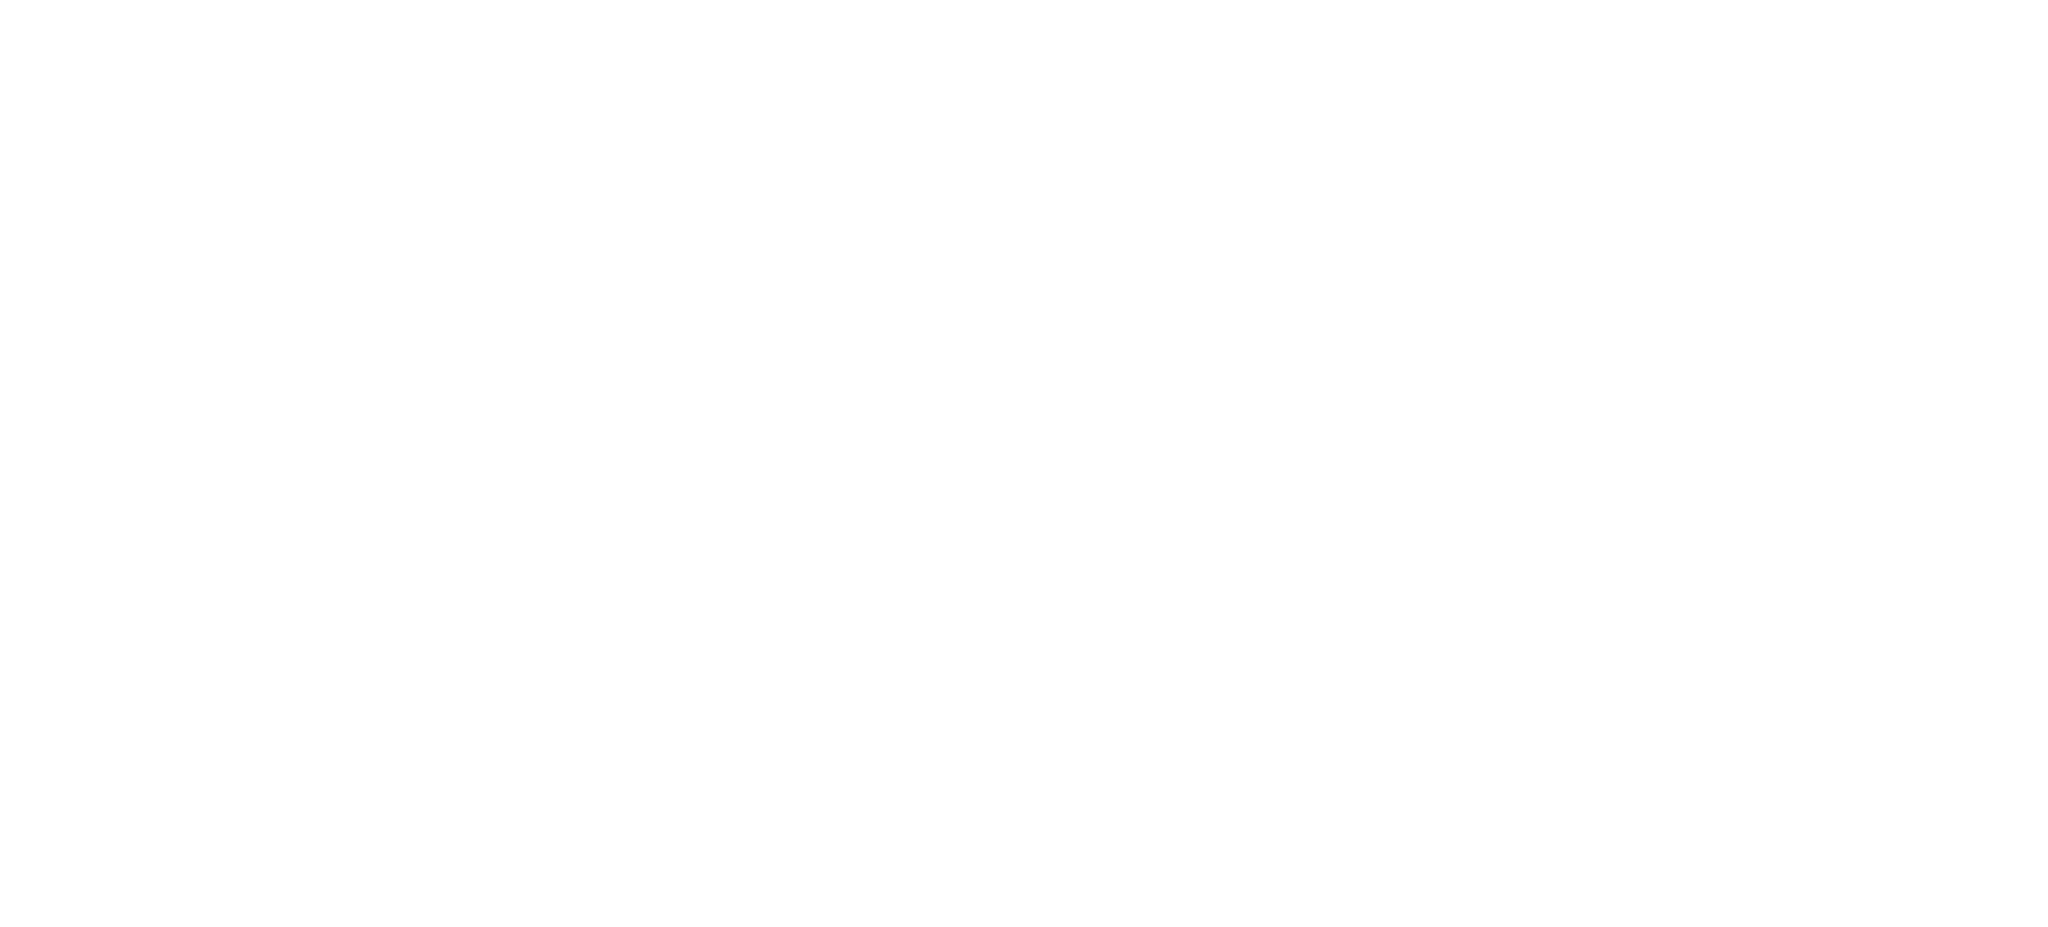
\includegraphics[width=0.85\textwidth]{cpu-add2.pdf}

\end{frame}


\begin{frame}
\frametitle{Add Immediate Value to register -- ADD}

\textbf{\texttt{addi} -- \texttt{addition immediate}} -- add immediate constat value to register and store result into destion register

\bigskip

\begin{tabular}{|l|l|}\hline
Description & Add rs1 and imm12 value and store result into rd \\ \hline
Operation& \texttt{[rd]} $\leftarrow$ \texttt{[rs1] + imm12} \\ \hline
Syntax & addi rd, rs1, imm12 \\ \hline
Encoding & \texttt{iiii iiii iiii ssss s000 dddd d001 0011} \\
 & i -- immediate; s -- rs1; d -- rd \\ \hline
\end{tabular}

\bigskip

Example: Increment register 7 value by 4 (store result into sama register 7 as is source):\\
\textbf{\texttt{addi x7, x7, 4}}

\textbf{\texttt{\color{red}iiii iiii iiii}}\phantom{xx}\textbf{\texttt{\color{blue}ssss s}}\hspace{0.1cm}\textbf{\texttt{000\hspace{0.25cm}{\color{green}dddd d}\hspace{0.05cm}001 0011}}\\
$\underbrace{\textbf{\texttt{\color{red}0000 0000 0100}}}_{0x004}\texttt{ }\underbrace{\textbf{\texttt{\color{blue}0011 1}}}_{7}\underbrace{\textbf{\texttt{000}}}_{func3}\phantom{i}\underbrace{\textbf{\texttt{\color{green}0011 1}}}_{7}\underbrace{\textbf{\texttt{001 0011}}}_{opcode}$\\

\textbf{\texttt{0x 00 43 83 93}} -- machine code \textbf{\texttt{addi x7, x7, 4}}


\end{frame}


\begin{frame}[shrink=10]
\frametitle{Operations with Immediate Value -- ADDI, ORI, ANDI}

\textbf{\texttt{addi} -- \texttt{add immediate}}: \texttt{[rd]} $\leftarrow$ \texttt{[rs1] + imm12} -- add immediate constat value \texttt{imm} to register \texttt{rs1} and store result into destion register \texttt{rd}

\bigskip

\begin{table}
\footnotesize
\begin{tabular}{|m{0.4cm}|m{0.4cm}|m{1.0cm}|m{1.0cm}|m{0.4cm}|m{1.0cm}|m{1.0cm}|m{1.0cm}|m{0.4cm}|m{1.0cm}|}\hline
Typ & 31 & 30...25 & 24...21 & 20 & 19...15 & 14...12 & 11...8 & 7 & 6...0 \\ \hline
I & \multicolumn{4}{c|}{ imm[11:0] } & rs1 & fnct3 &\multicolumn{2}{c|}{ rd } & opcode\\ \hline
\end{tabular}
\end{table}

\bigskip

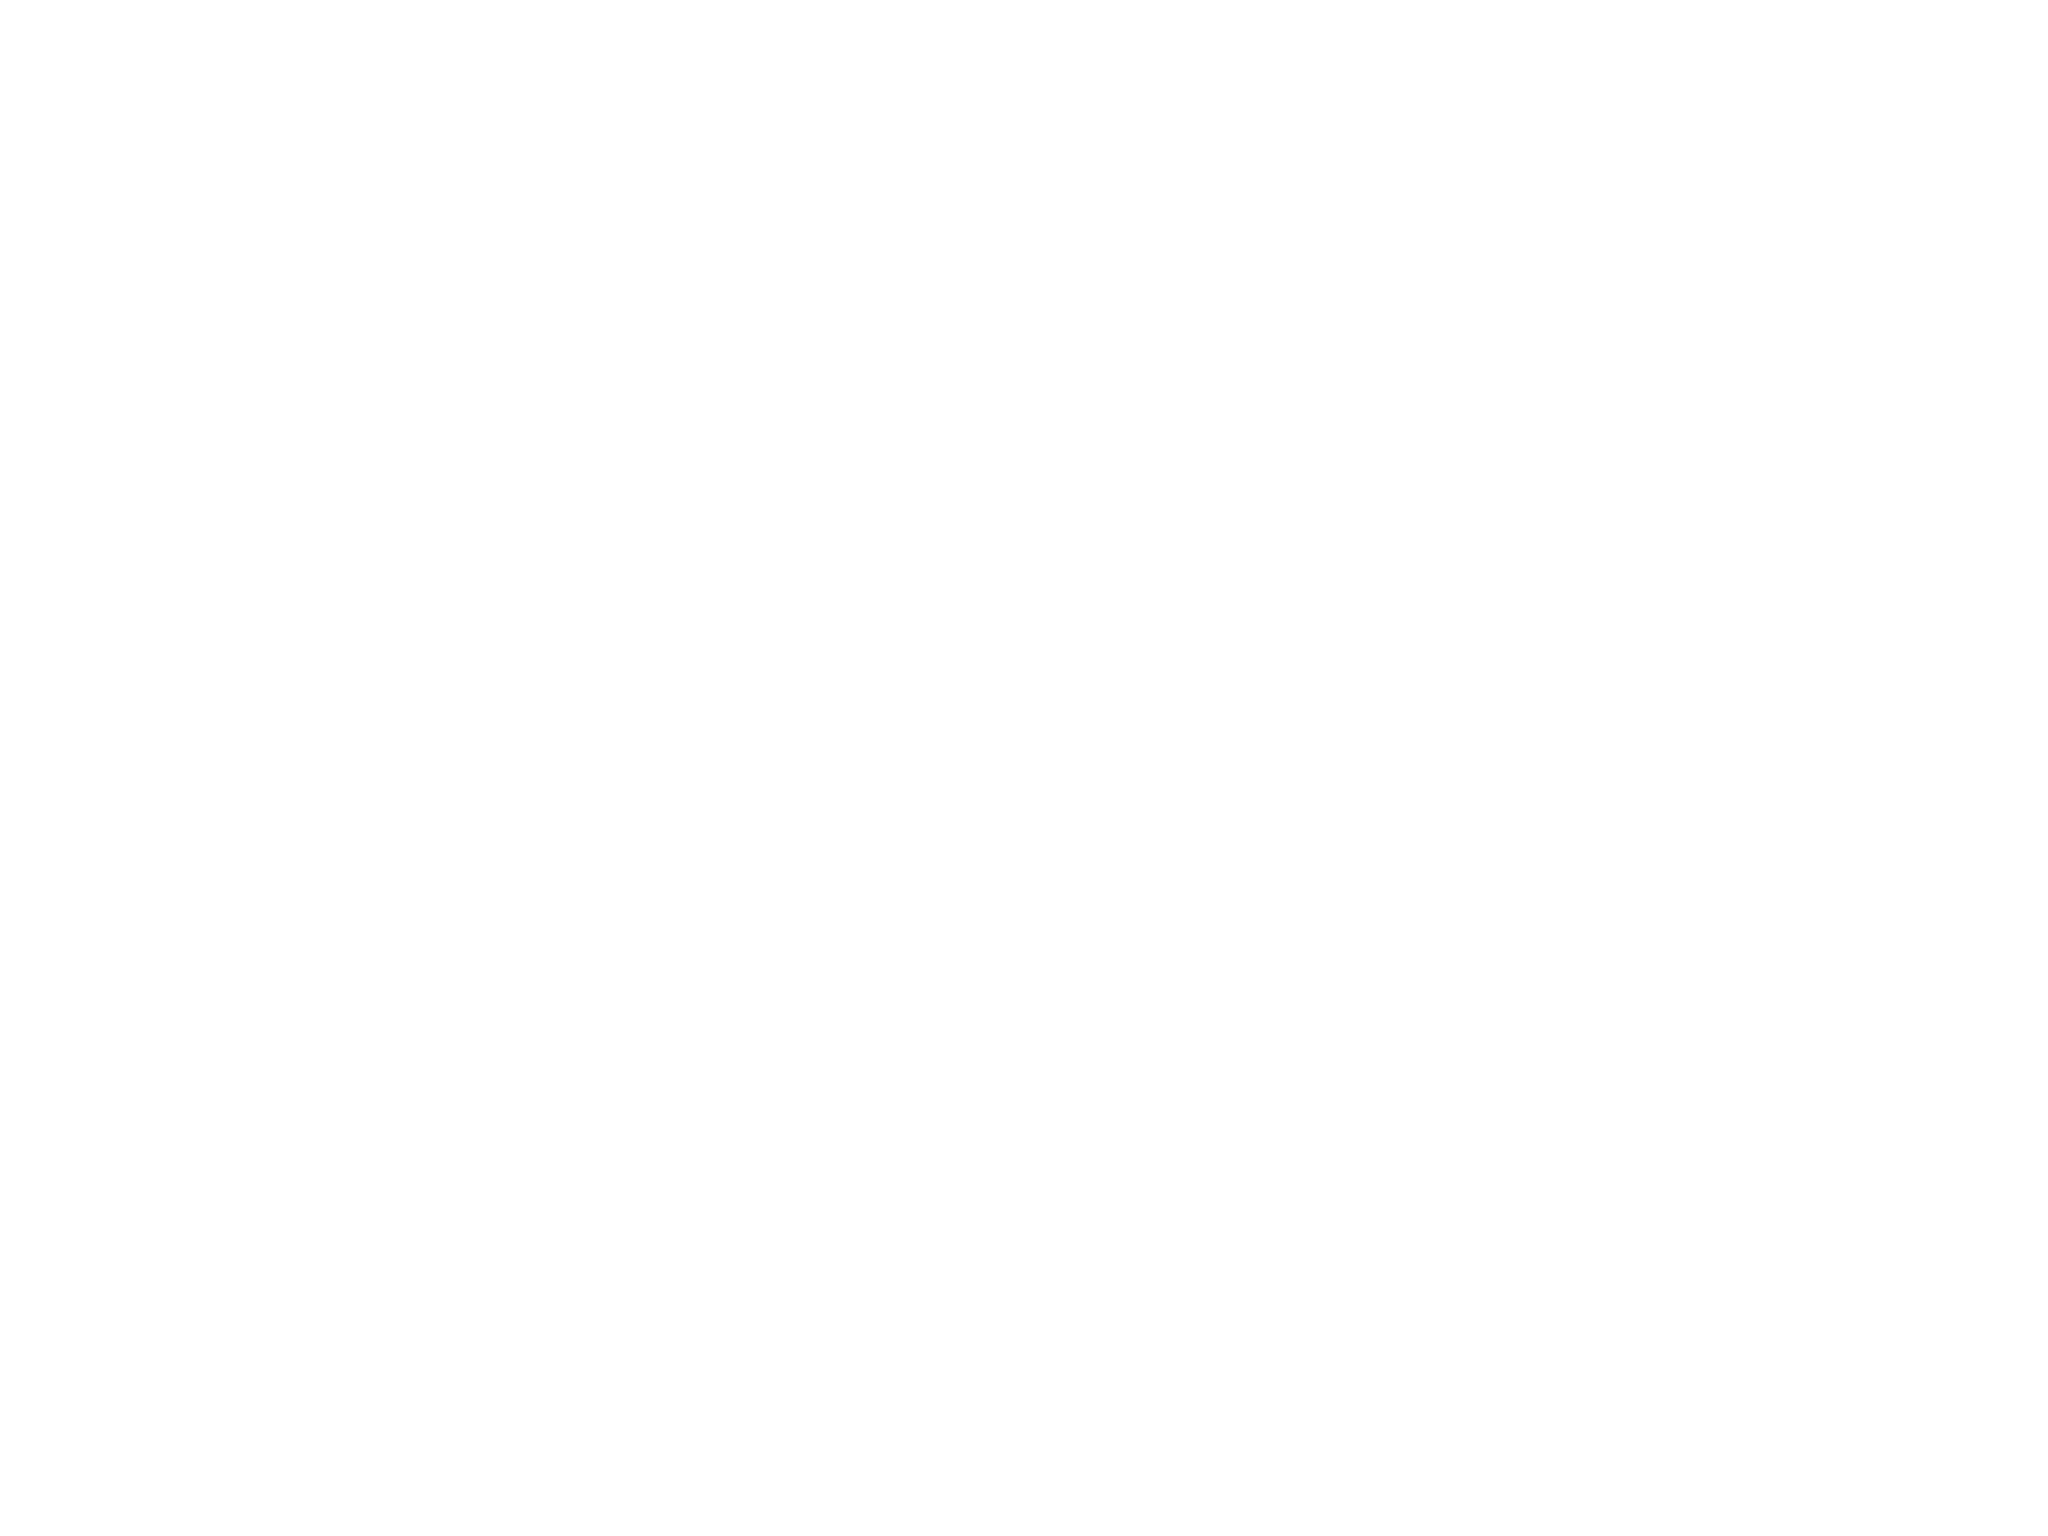
\includegraphics[width=0.85\textwidth]{cpu-addi.pdf}

\end{frame}


\begin{frame}[shrink=15]
\frametitle{Branch on Equal Instruction -- BEQ}

\textbf{\texttt{beq} -- \texttt{branch if equal}}: \texttt{[pc]} $\leftarrow$ \texttt{[pc] + SignImm} -- adds offset \texttt{imm} in the range -4096 to +4094 to the actual instruction address (\texttt{pc}) and continue execution at that address \texttt{pc} if the values stored in \texttt{rs1} and \texttt{rs2} are equal

\bigskip

\begin{table}
\footnotesize
\begin{tabular}{|m{0.4cm}|m{0.4cm}|m{1.0cm}|m{1.0cm}|m{0.4cm}|m{1.0cm}|m{1.0cm}|m{1.0cm}|m{0.4cm}|m{1.0cm}|}\hline
Typ & 31 & 30...25 & 24...21 & 20 & 19...15 & 14...12 & 11...8 & 7 & 6...0 \\ \hline
B & imm [12] & imm [10:5]  & \multicolumn{2}{c|}{ rs2 } & rs1 & fnct3 & imm[4:1]& imm [11] & opcode\\ \hline
\end{tabular}
\end{table}

\bigskip

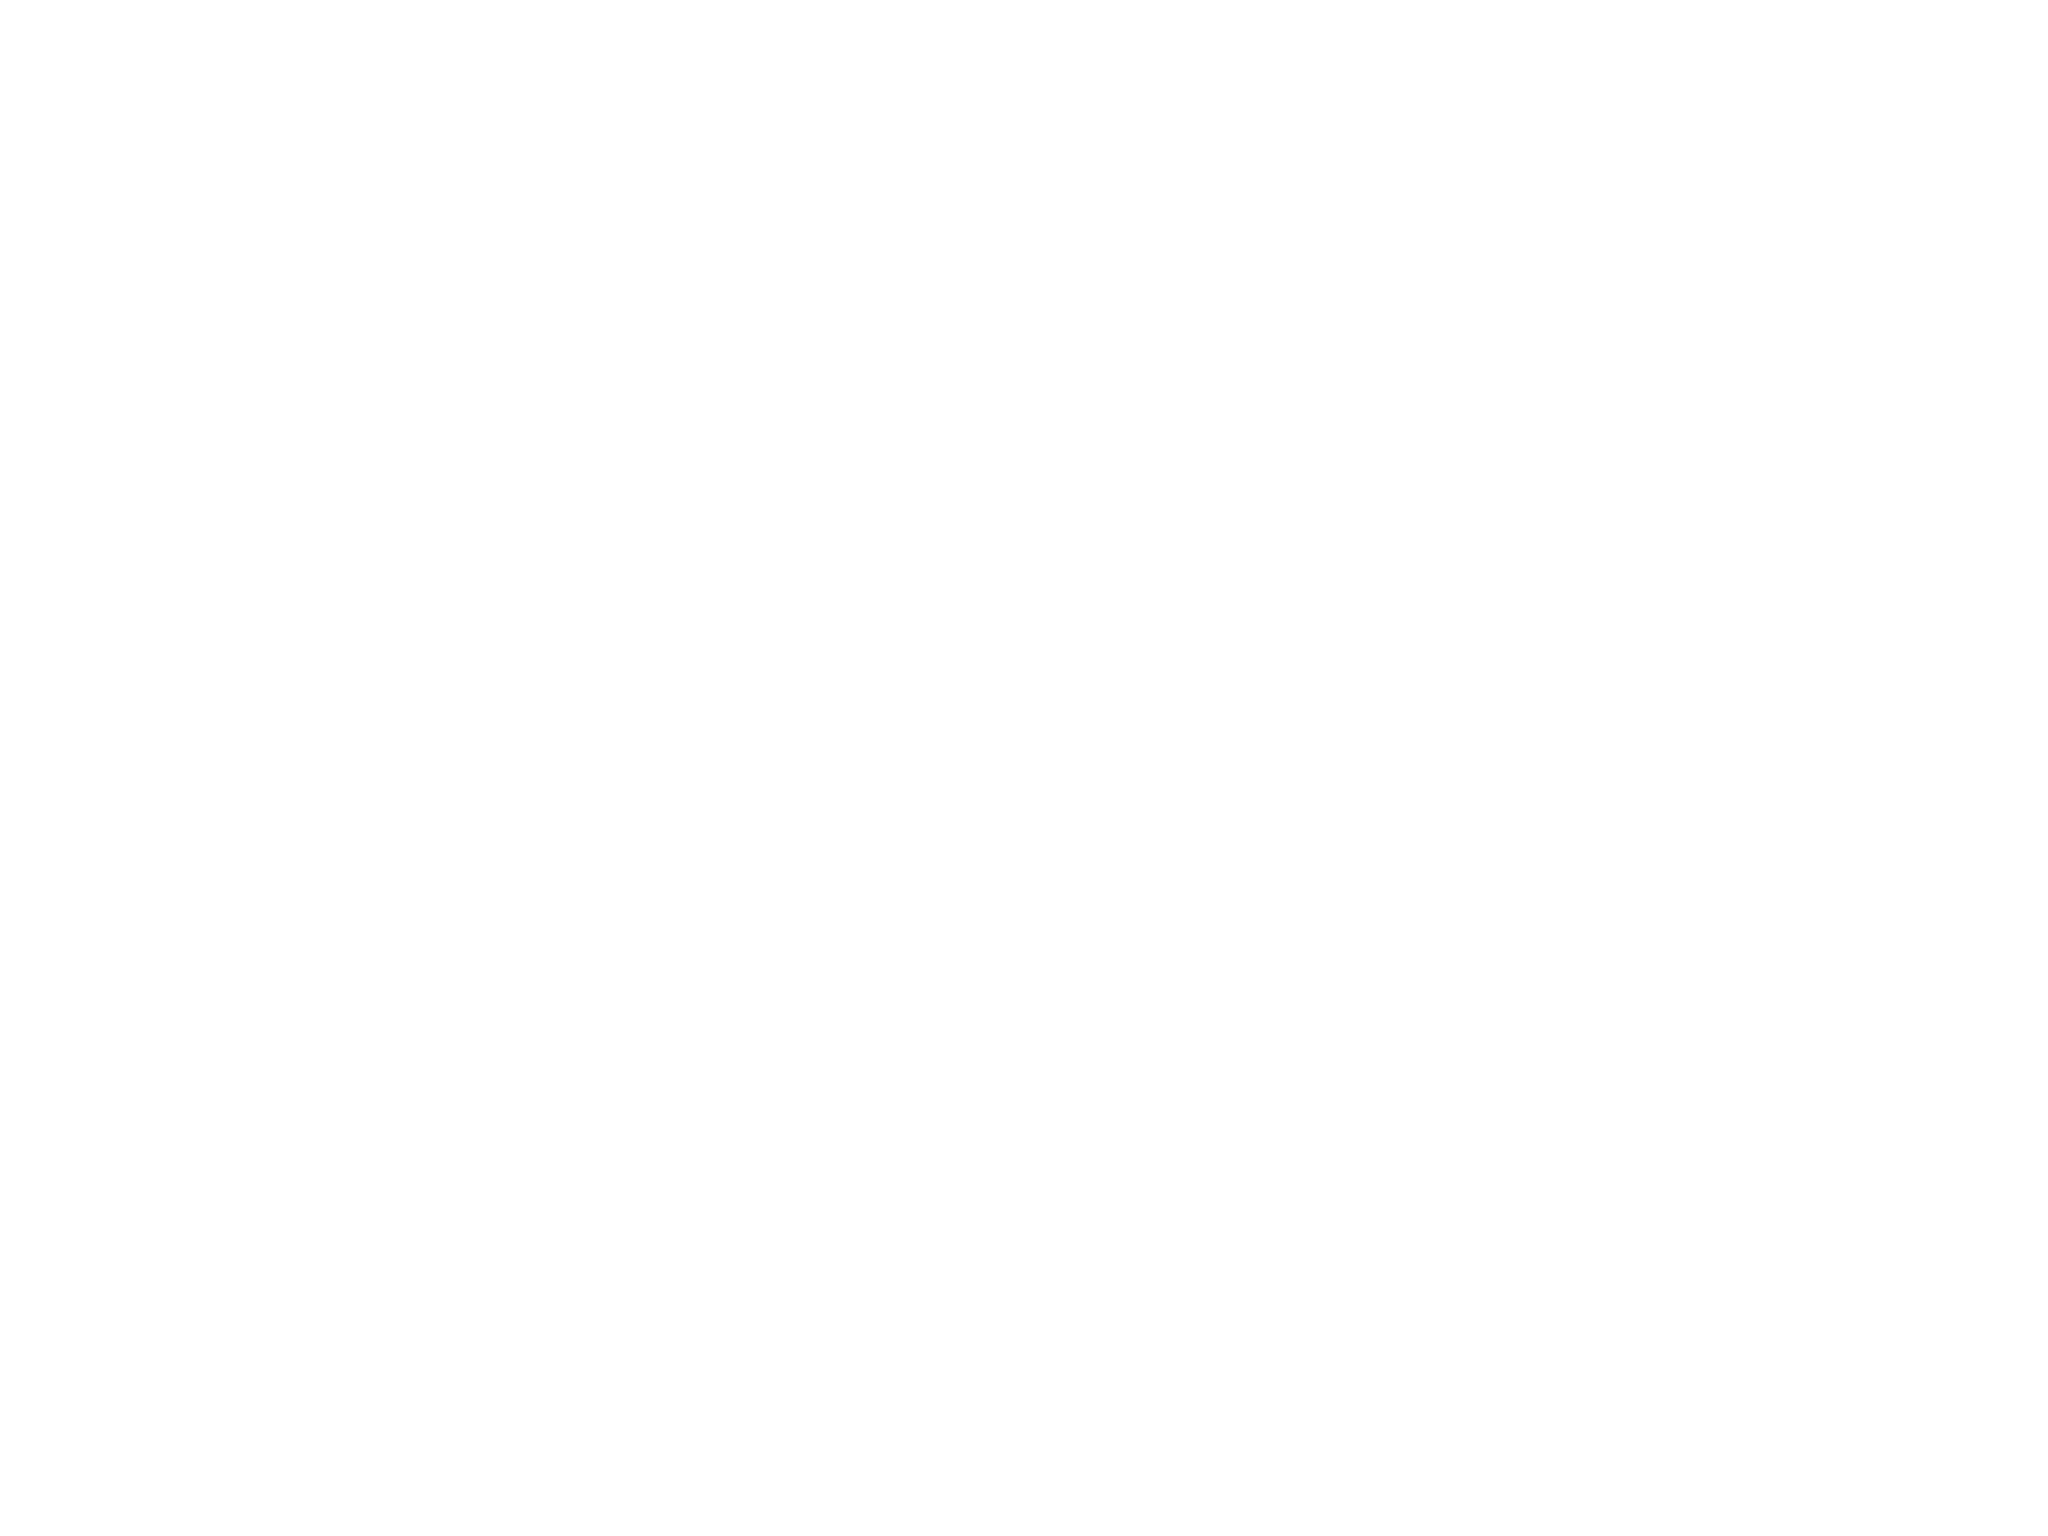
\includegraphics[width=0.85\textwidth]{cpu-beq.pdf}

\end{frame}


\begin{frame}
\frametitle{Single cycle CPU – Throughput: IPS = IC / T}

\bigskip

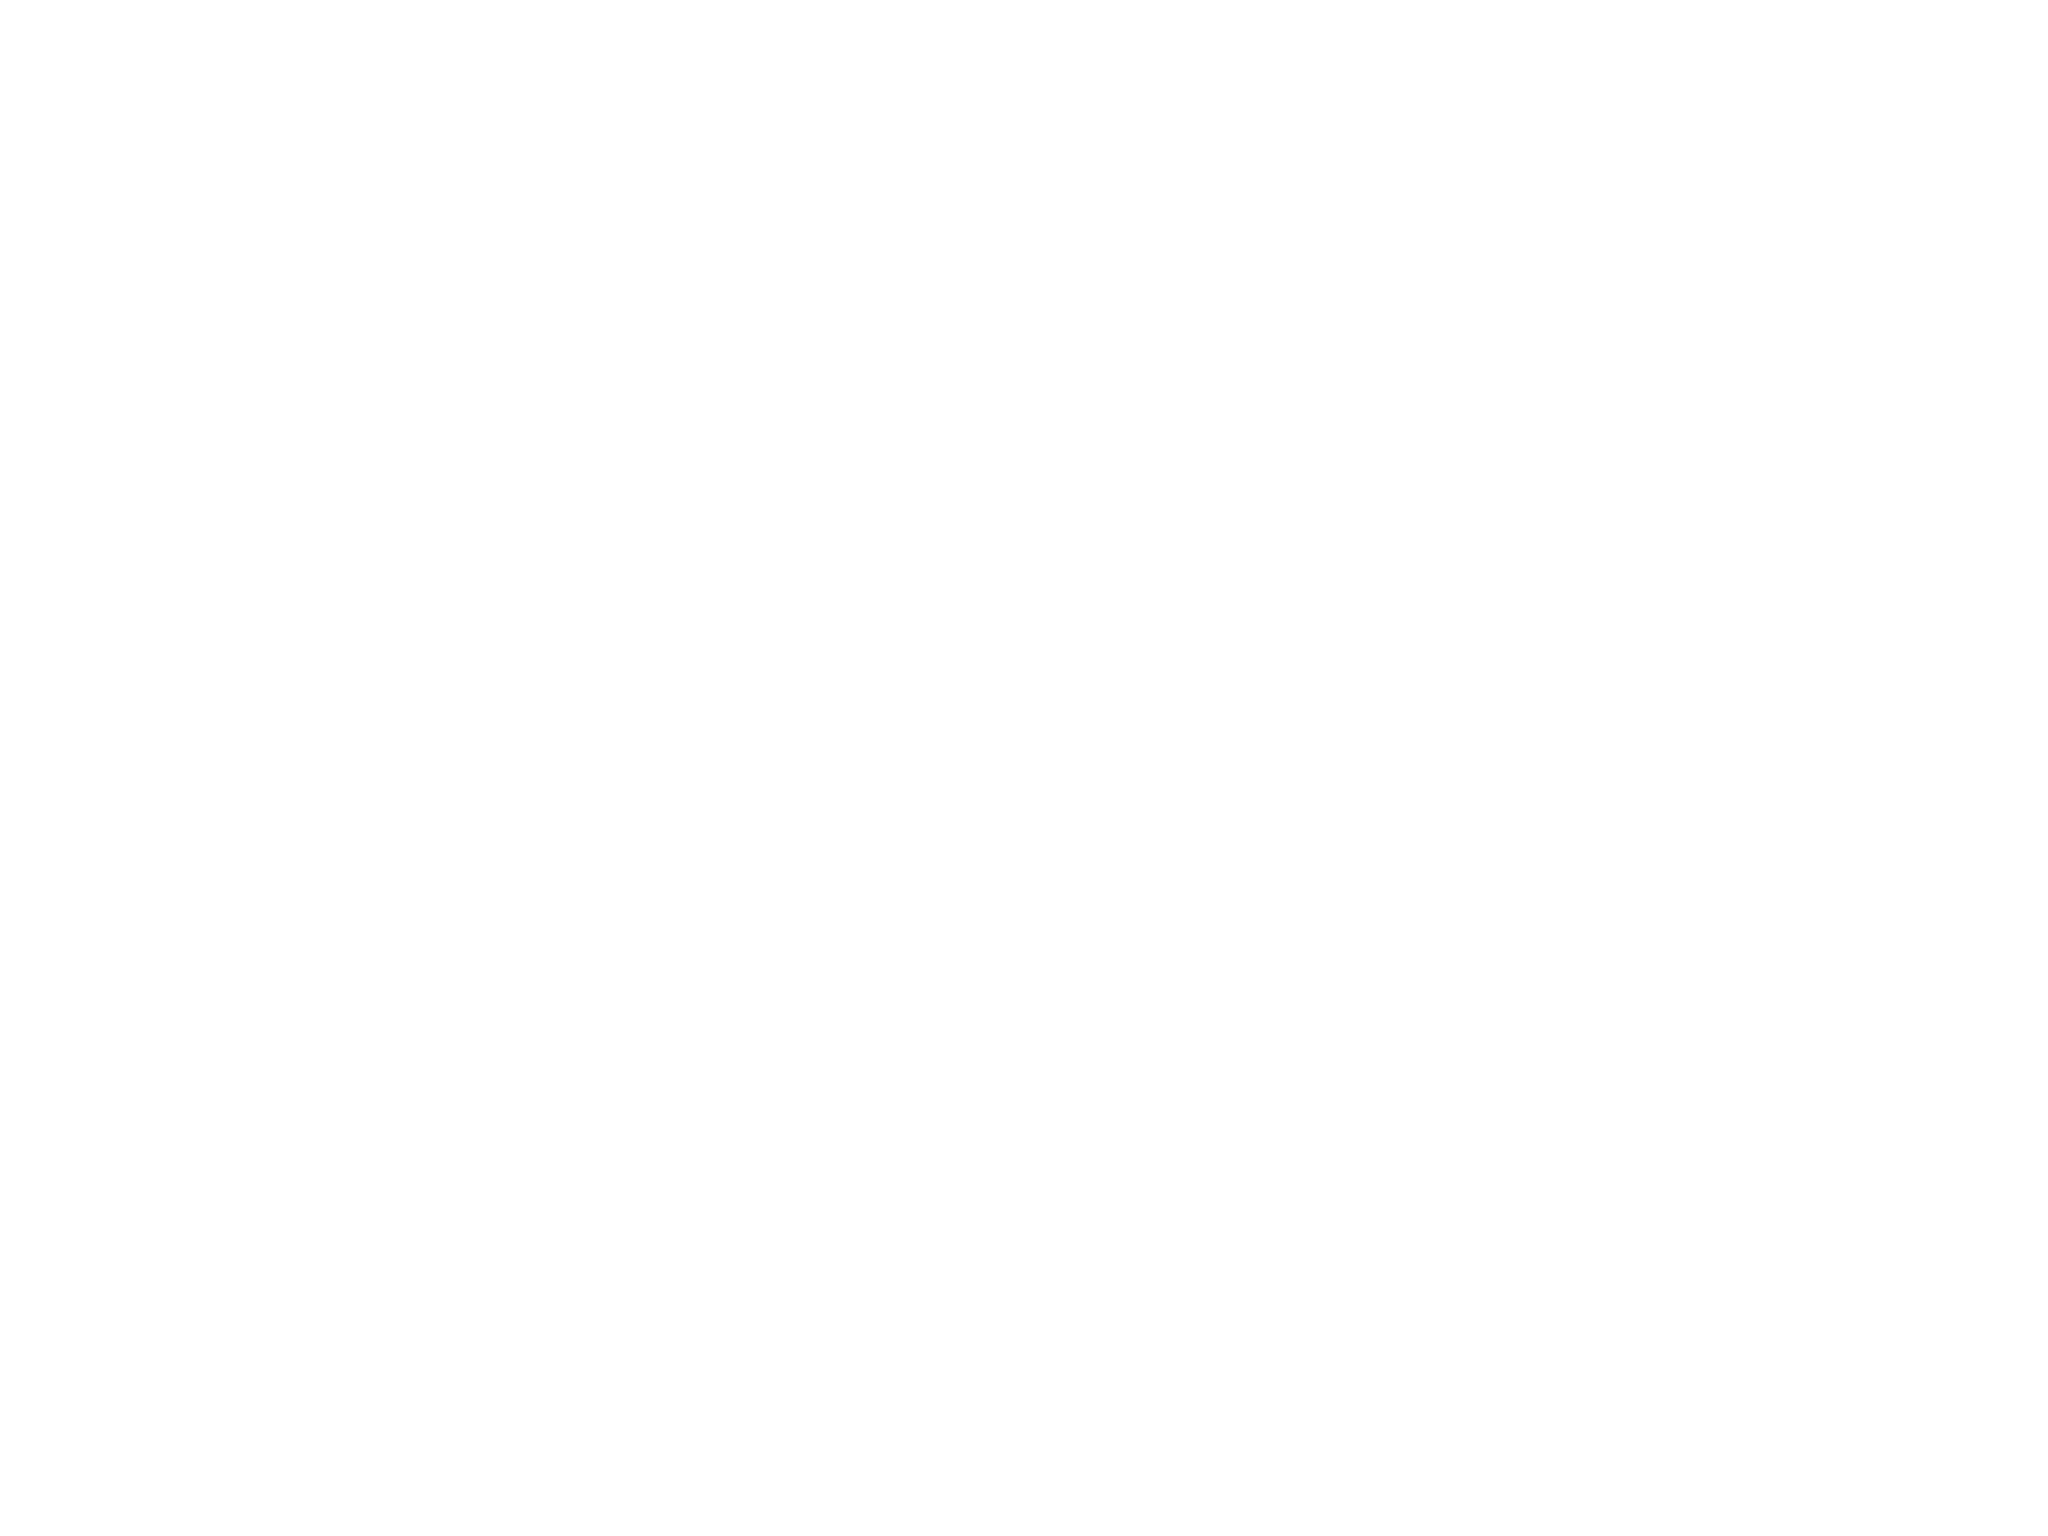
\includegraphics[width=0.85\textwidth]{cpu-time.pdf}

\end{frame}

\begin{frame}
\frametitle{Single cycle CPU – Longest Path}

What is the maximal possible frequency of the CPU?
\begin{itemize}
\item The all combinational circuits in the longest path has to settle (propagate values) with enough setup time, the worst case is \texttt{\textbf{lw}} instruction:
\begin{itemize}
\item $t_{PC} = 0,3$ ns
\item $t_{Mem} = 20$ ns
\item $t_{RFread} = 1,5$ ns
\item $t_{ALU} = 2$ ns
\item $t_{Mux} = 0,1$ ns
\item $t_{RFsetup} = 0,1$ ns
\end{itemize}
\item The sum for the longest cycle $T_{CLK} = t_{PC} + t_{Mem} + t_{RFread} + t_{ALU} + t_{Mem} + t_{Mux} + t_{RFsetup} = 44$ ns
\item The corresponding frequency $f_{CLK} = \frac{1}{T_{CLK}} = 22,7$ MHz, that is 22\,700\,000 instructions per seconds = 22,7 MIPS
\item We need to speedup execution, the topics for lecture 5
\end{itemize}
\end{frame}


\begin{frame}
\frametitle{Processor Control Unit -- Purpose}

It transform machine instruction bits \texttt{\textbf{opcode}} and \texttt{\textbf{fnct3,7}} to the control signals ALUControl, RegWrite, MemWrite, ALUSrc, MemToReg, Branch and some more for complete CPU

\bigskip
\begin{center}
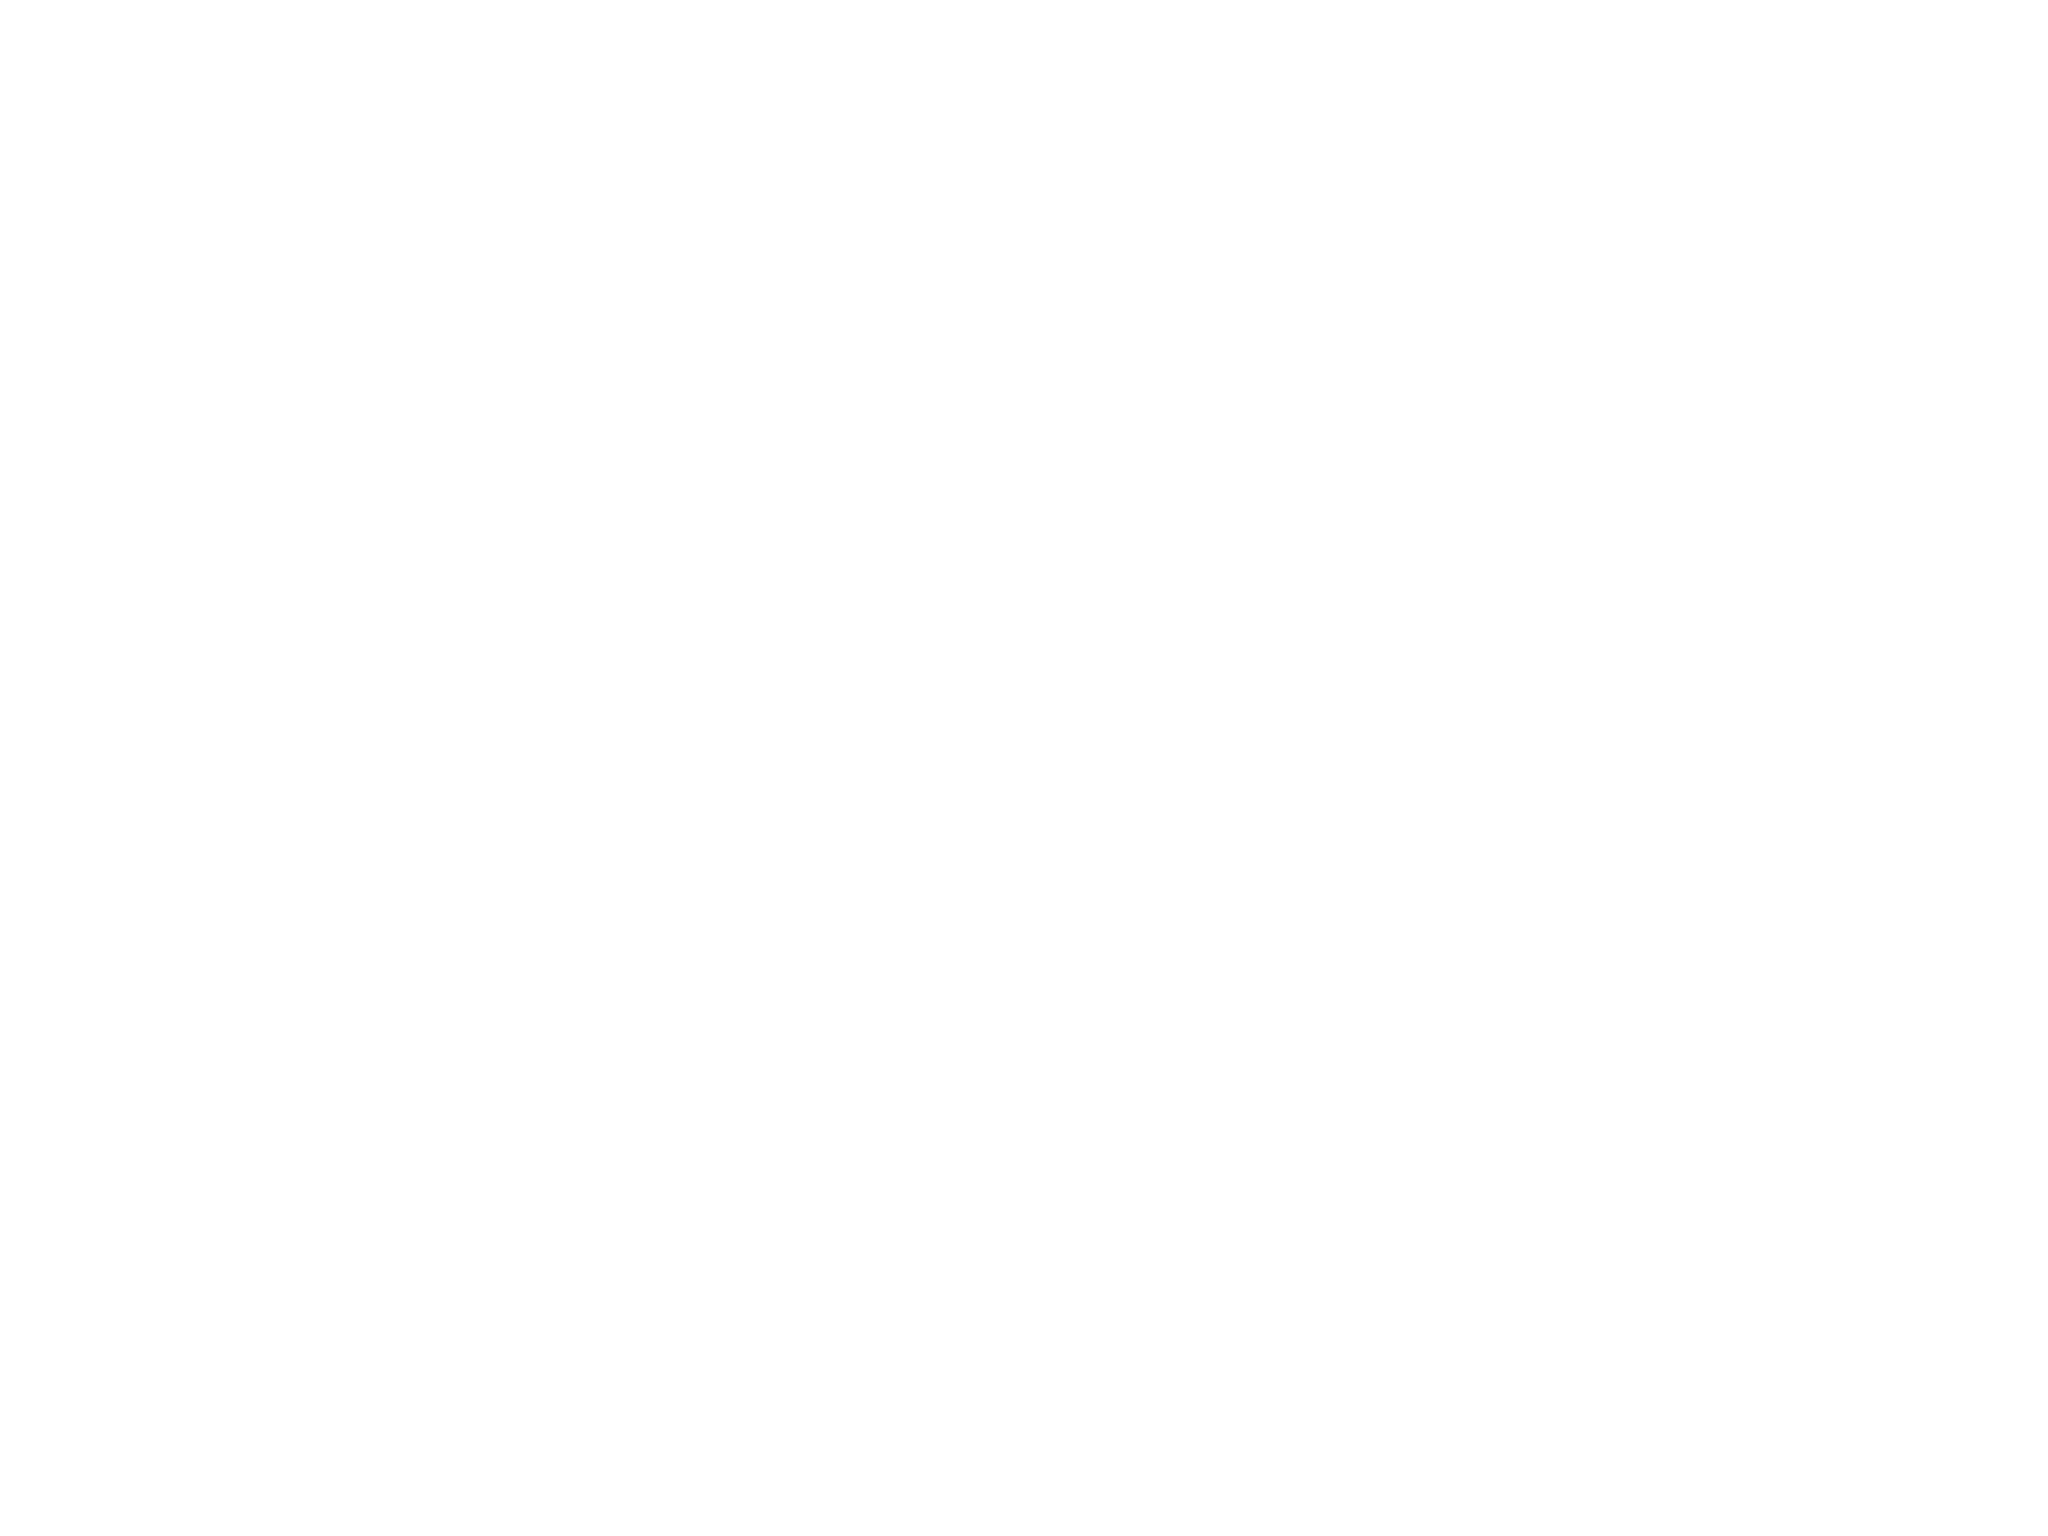
\includegraphics[width=0.75\textwidth]{cpu-control-unit.pdf}
\end{center}
\end{frame}

\begin{frame}
\frametitle{Processor Control Unit -- Implementation}

Podle Opcode lze nadefinovat výstupy řadiče:
\begin{tabular}{|lccc|cccccc|}\hline
Instruction & Opcode & Fnct3 & Fnct7 & \rotatebox{90}{ALUControl\phantom{x}} & \rotatebox{90}{ALUSrc} & \rotatebox{90}{RegWrite} & \rotatebox{90}{MemWrite} & \rotatebox{90}{MemToReg} & \rotatebox{90}{Branch} \\ \hline
lw & 0000011 & 010 & --       &           + & 1 & 1 & 0 & 1 & 0\\
sw & 0100011 & 010 & --       &           + & 1 & 0 & 1 & 0 & 0\\
add & 0110011 & 000 & 0000000 &           + & 0 & 1 & 0 & 0 & 0\\
sub & 0110011 & 000 & 0100000 &           - & 0 & 1 & 0 & 0 & 0\\
slt & 0110011 & 010 & 0000000 & \texttt{<} & 0 & 1 & 0 & 0 & 0\\
or & 0110011 & 110 & 0000000  & \texttt{|}  & 0 & 1 & 0 & 0 & 0\\
and & 0110011 & 111 & 0000000 & \texttt{\&} & 0 & 1 & 0 & 0 & 0\\
addi & 0010011 & 000 & --     &           + & 1 & 1 & 0 & 0 & 0\\
beq & 1100011 & 000 & --      & \texttt{==} & 0 & 0 & 0 & x & 1\\ \hline
\end{tabular}
\end{frame}


\begin{frame}[shrink=5]
\frametitle{Possible Ways to Implement Control Unit}
\begin{itemize}
\item Realized directly by a logic circuit design:
\begin{itemize}
\item Combinational logic (our example),
\item Sequential logic circuit - state machine, etc.
\end{itemize}
\item Microprogrammed control unit (controller by microprogram):
\begin{itemize}
\item The microprogram is stored in the control memory of the controller and consists of microinstructions.
\item The microprogram implements machine instructions visible to the programmer (add, sub, lw, xor, jmp,. . . ).
\item The instruction opcode specifies the address of the first microinstruction in control memory from which the microprogram for that instruction begins.
\item Each of the ISA instructions is executed using one or more microinstructions.
\item Advantage: a controller flexibility: ISA can be updated, extended by changing the microprogram
\item Disadvantages: more complex and unsuitable for pipelined processors where each stage executes a different instruction. Today used for sequential translation of such CISC instructions which are too complex to be translated into one or more RISC like microoperations directly by combinational logic
\end{itemize}
\end{itemize}
\end{frame}


\end{document}

